%\documentclass[notes,handout,11pt,aspectratio=169]{beamer}
%\documentclass[notes,11pt,aspectratio=169]{beamer}

% The following creates extra wide pages containing the main
% slide and any accompanying notes next to it.
%\usepackage{pgfpages}\setbeameroption{show notes on second screen=right}


\documentclass[11pt,aspectratio=169]{beamer}


\usepackage{epsfig}

% use serif fonts in math mode
\usefonttheme[onlymath]{serif}

\usepackage{verbatim,comment,ifthen}
\usepackage{tikz}
\usetikzlibrary{calc}
\usepackage{graphicx}
\usepackage{mdframed,alltt}

\usepackage{listings}

%,alltt,multicol,epsfig,color,fancyvrb}


%%-----------------------------------------
%% Shortcuts ...
%%-----------------------------------------
\newcommand{\bi}{\begin{itemize}}
\newcommand{\ei}{\end{itemize}}

\newcommand{\be}{\begin{enumerate}}
\newcommand{\ee}{\end{enumerate}}

\newcommand{\x}{\item}
%%-----------------------------------------
\newcommand{\eedd}{\end{document}}

\newcommand{\isize}[1]{\setlength{\itemsep}{#1}}

\newcommand{\bis}[1]{\begin{itemize}\setlength{\itemsep}{#1}}
\newcommand{\bes}[1]{\begin{enumerate}\setlength{\itemsep}{#1}}


\newcommand{\biA}{\bis{0.5cm}}
\newcommand{\biB}{\bis{0.65cm}}
\newcommand{\biC}{\bis{0.8cm}}
\newcommand{\biZ}{\bis{0cm}}
\newcommand{\beA}{\bes{0.5cm}}
\newcommand{\beB}{\bes{0.65cm}}
\newcommand{\beC}{\bes{0.8cm}}

\newcommand{\myitem}[2]{\item{#1}\note[item]{#2}}


\setbeamerfont{itemize/enumerate body}{}
\setbeamerfont{itemize/enumerate subbody}{size=\normalsize}
\setbeamerfont{itemize/enumerate subsubbody}{size=\normalsize}


\newcommand{\eg}{\emph{e.g.}}

\newcommand\vskipA{\vskip 0.5cm}
\newcommand\vskipB{\vskip 0.75cm}


%\newcommand{\alert}[1]{\textbf{#1}}
\newcommand{\triple}[3]{\ensuremath{\{#1\}}\ \code{#2}\ \ensuremath{\{#3\}}}

%% Symbols
\newcommand{\ttlbrace}{\mbox{\tt\symbol{123}}}
\newcommand{\ttrbrace}{\mbox{\tt\symbol{125}}}
\newcommand{\ttlbracket}{\mbox{\tt\symbol{133}}}
\newcommand{\ttrbracket}{\mbox{\tt\symbol{135}}}
\newcommand{\ttbackslash}{\mbox{\tt\symbol{92}}}
\newcommand{\tthat}{\mbox{\tt\symbol{94}}}
\newcommand{\ttat}{\mbox{\tt\symbol{64}}}
\newcommand{\tttilde}{\mbox{\tt\symbol{126}}}
\newcommand{\kwd}[1]{\textbf{#1}}

\newcommand{\back}{\ensuremath{\backslash}}
\newcommand{\defas}{\triangleq}


%% Counters
\newcounter{backupcounter}
\newcounter{exercounter}
\setcounter{exercounter}{0}



%% Colors
\setbeamercolor{redcolor}{fg=red}
\newcommand{\hir}[1]{{\usebeamercolor[fg]{redcolor}#1}}


\setbeamercolor{bluecolor}{fg=blue}

\definecolor{dgreen}{rgb}{0.0,0.6,0.0}
\definecolor{dblue}{rgb}{0.0,0.0,1.0}
\definecolor{whilte}{rgb}{0.0,0.0,0.0}

%\newcommand{\hib}[1]{{\usebeamercolor[fg]{bluecolor}#1}}

\newcommand{\hib}[1]{{\textcolor{dblue}{#1}}}
\newcommand{\hig}[1]{{\textcolor{dgreen}{#1}}}
\newcommand{\hiw}[1]{{\textcolor{white}{#1}}}

%\newcommand{\code}[1]{\texttt{\usebeamercolor[fg]{bluecolor}#1}}
%\newcommand{\code}[1]{\texttt{\hig{#1}}}
\newcommand{\code}[1]{\texttt{\hib{#1}}}
\newcommand{\nt}[1]{\ensuremath{\langle\mathit{#1}\rangle}}
\newcommand{\term}[1]{\ensuremath{\mathit{#1}_t}}
\newcommand{\termlit}[1]{``\ensuremath{\mathit{#1}}''}

%\newcommand{\frametitle}[1]{}

%\newcommand{\ftitle}[1]{\renewcommand{\frametitle}{#1}}

%% Environments - default setting, modified in
%% task_(screen|guide|notes).tex



\newcommand{\pnum}{Slide \#\arabic{framenumber}}
\newcommand{\nonotes}{\note{\pnum{} No notes for this slide}}
\newcommand{\guideonly}[1]{\mode<handout>{#1}}

%\newcommand{\

\newenvironment{exercise}[1]{\stepcounter{exercounter}%
    \begin{frame}[containsverbatim,t]{Exercise \#\arabic{exercounter}: #1}}{\end{frame}}

%\newenvironment{exercise}[1]{\stepcounter{exercounter}%
%    \begin{frame}<beamer|notes>[t]{Exercise \#\arabic{exercounter}:#1}}{\end{frame}}


% set up footer with frame number
\setbeamertemplate{footline}[text line]{%
 \parbox{\linewidth}{\vspace*{-8pt}\hfill\insertframenumber}}

% hide those navigation symbols
\setbeamertemplate{navigation symbols}{} 


%
% Note page template
% ---- ---- --------
%
\setbeamertemplate{note page}{%
%\begin{minipage}[c]{0.6\textwidth}

\textbf{Note.} \hib{\insertframetitle{}}
\insertframenumber{} / \inserttotalframenumber 

%\end{minipage}
%\begin{minipage}[c]{0.39\textwidth}
%\insertslideintonotes{0.5}
%\end{minipage}

%\begin{figure}
%\insertslideintonotes{0.25}
%\end{figure}

% 720p in 3-111
% 12x8 in Tate

%{\footnotesiz

\insertnote

}

\newcommand{\nonote}{\note{No Note. \\ \insertslideintonotes{0.85}}}
\newcommand{\stopcounting}{\setcounter{backupcounter}{\value{framenumber}}}
\newcommand{\startcounting}{\setcounter{framenumber}{\value{backupcounter}}}


\newcommand{\exts}[1]{\texttt{\hig{#1}}}


\lstset{escapeinside={(*@}{@*)},basicstyle=\small\ttfamily\color{blue}}

%\setlength{\leftmargini}{0.4cm}



\newcommand{\egray}[1]{{\usebeamercolor[fg]{graycolor}#1}}
\setbeamercolor{whitecolor}{fg=white}
\newcommand{\ewhite}[1]{{\usebeamercolor[fg]{whitecolor}#1}}
\newcommand{\tcode}[1]{\hib{\texttt{#1}}}

\setbeamercolor{greencolor}{fg=dgreen}
\newcommand{\egreen}[1]{{\usebeamercolor[fg]{greencolor}#1}}

\newboolean{showanim}\setboolean{showanim}{true}



\setbeamercolor{bluecolor}{fg=blue}
\newcommand{\eblue}[1]{{\usebeamercolor[fg]{bluecolor}#1}}
\setbeamercolor{blackcolor}{fg=black}
\newcommand{\eblack}[1]{{\usebeamercolor[fg]{blackcolor}#1}}
\newcommand{\eorange}[1]{{\usebeamercolor[fg]{orangecolor}#1}}
\setbeamercolor{orangecolor}{fg=orange}

\setbeamercolor{redcolor}{fg=red}
\newcommand{\ered}[1]{{\usebeamercolor[fg]{redcolor}#1}}

% used only in challenges in scanning
\newcommand{\codesblue}[1]{\small{\texttt{\eblack{#1}}}}
\newcommand{\codesblack}[1]{\small{\texttt{\eblue{#1}}}}

\newcommand{\betable}{DNF\_table\_kwd}

\newcommand{\ableC}{\textsc{ableC}}
\newcommand{\silver}{\textsc{Silver}}


% Attribution animation commands
\newcommand{\ys}{1.3}

\newcommand{\enve}[2]{\draw[blue] ($(#1-0.4,\ys*#2-0.35)$) circle(0.15);}
\newcommand{\envd}[2]{\filldraw[blue] ($(#1-0.4,\ys*#2-0.35)$) circle(0.05);}
\newcommand{\envc}[2]{\filldraw[blue] ($(#1-0.4,\ys*#2-0.35)$) circle(0.15);}

\newcommand{\ppe}[2]{\draw[dgreen] ($(#1+0.4,\ys*#2-0.35)$) circle(0.15);}
\newcommand{\ppd}[2]{\filldraw[dgreen] ($(#1+0.4,\ys*#2-0.35)$) circle(0.05);}
\newcommand{\ppc}[2]{\filldraw[dgreen] ($(#1+0.4,\ys*#2-0.35)$) circle(0.15);}

\newcommand{\vale}[2]{\draw[red] ($(#1+0.8,\ys*#2-0.35)$) circle(0.15);}
\newcommand{\vald}[2]{\filldraw[red] ($(#1+0.8,\ys*#2-0.35)$) circle(0.05);}
\newcommand{\valc}[2]{\filldraw[red] ($(#1+0.8,\ys*#2-0.35)$) circle(0.15);}

\newcommand{\erre}[2]{\draw[orange] ($(#1+1.2,\ys*#2-0.35)$) circle(0.15);}
\newcommand{\errd}[2]{\filldraw[orange] ($(#1+1.2,\ys*#2-0.35)$) circle(0.05);}
\newcommand{\errc}[2]{\filldraw[orange] ($(#1+1.2,\ys*#2-0.35)$) circle(0.15);}

\newcommand{\pptopp}[4]
{\draw[dgreen,->] ($(#1+0.4,\ys*#2-0.35)$) -- ($(#3+0.4,\ys*#4-0.35)$);}
\newcommand{\pptoppw}[4]
{\draw[white,->] ($(#1+0.4,\ys*#2-0.35)$) -- ($(#3+0.4,\ys*#4-0.35)$);}

\newcommand{\envtoenv}[4]
{\draw[blue,->] ($(#1-0.4,\ys*#2-0.35)$) -- ($(#3-0.4,\ys*#4-0.35)$); }

\newcommand{\envtoval}[4]
{\draw[blue,->] ($(#1-0.4,\ys*#2-0.35)$) -- ($(#3+0.8,\ys*#4-0.35)$); }

\newcommand{\valtoval}[4]
{\draw[red,->] ($(#1+0.8,\ys*#2-0.35)$) -- ($(#3+0.8,\ys*#4-0.35)$); }

\newcommand{\valtoenv}[4]
{\draw[red,->] ($(#1+0.8,\ys*#2-0.35)$) -- ($(#3-0.4,\ys*#4-0.35)$); }

\newcommand{\rtn}[3]{
% production
\draw ($(#1,#2*\ys)$) node{#3};
% pp
\ppe{#1}{#2}
% val
\vale{#1}{#2}
% errors
%\erre{#1}{#2}

\draw[gray] ($(#1+0.65,\ys*#2+0.25)$) --
            ($(#1-0.3,\ys*#2+0.25)$) arc (90:270:4.5mm);

\draw[gray] ($(#1+0.65,\ys*#2+0.25)$) arc (90:-90:4.5mm) -- 
            ($(#1-0.3,\ys*#2-0.65)$) ;
}

\newcommand{\rtnna}[3]{
% production
\draw ($(#1,#2*\ys)$) node{#3};
% pp
%\ppe{#1}{#2}
% val
%\vale{#1}{#2}
% errors
%\erre{#1}{#2}

\draw[gray] ($(#1+0.65,\ys*#2+0.25)$) --
            ($(#1-0.3,\ys*#2+0.25)$) arc (90:270:4.5mm);

\draw[gray] ($(#1+0.65,\ys*#2+0.25)$) arc (90:-90:4.5mm) -- 
            ($(#1-0.3,\ys*#2-0.65)$) ;
}

\newcommand{\tnna}[3]{
\rtnna{#1}{#2}{#3}
%\enve{#1}{#2}
}

\newcommand{\tn}[3]{
\rtn{#1}{#2}{#3}
\enve{#1}{#2}
}

\newcommand{\tnstr}[3]{
\draw ($(#1,#2*\ys)$) node{#3};
\draw[gray] ($(#1+0.25,\ys*#2+0.25)$) --
            ($(#1-0.2,\ys*#2+0.25)$) arc (90:270:2.5mm);

\draw[gray] ($(#1+0.25,\ys*#2+0.25)$) arc (90:-90:2.5mm) -- 
            ($(#1-0.2,\ys*#2-0.25)$) ;

}

\newcommand{\tedge}[4]{
\draw[gray] ($(#1+\xsh,\ys*#2-0.65)$) -- ($(#3+\xsh,\ys*#4+0.25)$);
}

\newcommand{\ppeval}{
% pp evaluation
\pause
\ppd{4}{4} %root
\pause
\ppd{4}{3} %let

\pause
\ppd{4}{2} %true-let
\pause
\ppc{4}{2} %true-let
\pause
\ppd{6.5}{2}  %and

\pause
\ppd{5.25}{1} %true-and
\pause
\ppc{5.25}{1} %true-and
\pause
\ppd{7.75}{1} %ref
\pause
\ppc{7.75}{1} %ref

\pause
\ppc{6.5}{2}  %and

\pause
\ppc{4}{3} %let

\pause
\ppc{4}{4} %root
}

\newcommand{\valeval}{
% val evaluation
\pause\vald{4}{4} %root
\pause\vald{4}{3} %let

\pause\vald{6.5}{2}  %and
\pause\vald{5.25}{1} %true-and
\pause\valc{5.25}{1} %true-and

\pause\vald{7.75}{1} %ref

\pause\envd{7.75}{1} %ref

\pause\envd{6.5}{2}  %and

\pause
\draw ($(5.5,\ys*-0.5)$) node {\small\texttt{body.env = addEnv(name, dval.val, e.env);}};

\pause\vald{4}{2} %true-let
\pause\valc{4}{2} %true-let

\pause\envd{4}{3} %let
\pause\envc{4}{3} %let

\pause\envc{6.5}{2}  %and

\pause
\draw[white] ($(5.5,\ys*-0.5)$) node {\small\texttt{body.env = addEnv(name, dval.val, e.env);}};

\pause\envc{7.75}{1} %ref

\pause\valc{7.75}{1} %ref
\pause\valc{6.5}{2}  %and

\pause\valc{4}{3} %let

\pause\valc{4}{4} %root
}

\newcommand{\xsh}{0.15}



\newcommand{\rtne}[3]{
% production
\draw ($(#1,#2*\ys)$) node{#3};
\ppe{#1}{#2}
\vale{#1}{#2}
\erre{#1}{#2}

\draw[gray] ($(#1+1.1,\ys*#2+0.25)$) --
            ($(#1-0.3,\ys*#2+0.25)$) arc (90:270:4.5mm);

\draw[gray] ($(#1+1.1,\ys*#2+0.25)$) arc (90:-90:4.5mm) -- 
            ($(#1-0.3,\ys*#2-0.65)$) ;
}

\newcommand{\tne}[3]{
\rtne{#1}{#2}{#3}
\enve{#1}{#2}
}

\newcommand{\ppevalimplies}{
\pause\ppc{6.5}{2} %implies

\ppc{5.25}{1} % imp-true
\ppc{7.75}{1}% imp-ref


}
\newcommand{\erroreval}{


%\errd{5.25}{1} % imp-true
%\errd{7.75}{1}% imp-ref

\pause\errd{11.5}{2} % or
\pause\errd{10.25}{1} % not
\pause\errd{10.25}{0} % or-true

\pause\errc{10.25}{0} % or-true
\pause\errc{10.25}{1} % not

\pause\errd{12.75}{1} % or-ref
\pause\envd{12.75}{1} % or-ref
\pause\envd{11.5}{2} % or

\pause\envd{6.5}{2} %implies
\pause\envc{6.5}{2} %implies

\pause\envc{11.5}{2} % or

\pause\envc{12.75}{1} % or-ref
\pause\errc{12.75}{1} % or-ref

\pause\errc{11.5}{2} % or

\pause\errc{6.5}{2} %implies

}


\newcommand{\showimplies}{
%\ifthenelse{\boolean{showanim}}{\errc{3.5}{0}\draw (5.5,-0.35) node{inline};}{}

% -0.4
\envc{1.4}{2}
\draw (1.65,2.2) node{env};

% +0.4
\ppc{0.6}{1.5}
\draw (1.65,1.5) node{pp};

% + 0.8
\valc{0.2}{1}
\draw (1.65,1.0) node{val};
% + 1.2
\errc{-0.2}{0.5}
\draw (1.9,0.35) node{inline};

%\envc{3}{3}
%\draw (3.9,3.85) node{env};

%\ppc{3}{2.5}
%\draw (3.84,2.5) node{pp};

%\valc{3}{0}
%\draw (4.88,0.6) node{val};




\tedge{5.5}{3}{6.5}{2}
\tne{6.5}{2}{\ \ implies}
\tedge{6.5}{2}{5.25}{1}
\tedge{6.5}{2}{7.75}{1}



\tne{5.25}{1}{true}

\tne{7.75}{1}{ref}
\tedge{7.75}{1}{7.75}{0}

\tnstr{7.85}{0}{"n"}

\ppevalimplies

\pause\errd{6.5}{2} %implies

\pause
\draw[thick,->] ($(8.25,\ys*1.85)$) -- ($(10.55,\ys*1.85)$);

\tne{11.5}{2}{or}
\tedge{11.5}{2}{10.25}{1}
\tedge{11.5}{2}{12.75}{1}

\tne{10.25}{1}{not}
\tedge{10.25}{1}{10.25}{0}

\tne{10.25}{0}{true}

\tne{12.75}{1}{ref}
\tedge{12.75}{1}{12.75}{0}

\tnstr{12.85}{0}{"n"}

\erroreval
}



\begin{document}

\begin{frame}
\begin{center}
%{\hib{\Large \textsc{ableC} Tutorial}}
%\vskip 0.75cm

{\Large\hib{Attribute Grammars in Silver}}

\vskip 0.25cm
{\large\hib{Composable and Modular Language Specifications}}

\vskip 1cm
Lucas Kramer and Eric Van Wyk

\medskip
University of Minnesota

\bigskip
August 26, 2022

\end{center}
\end{frame}

%\note{Attribute grammars were invented in 1968 by Donald Knuth as a formalism for specifying the semantics of context free languages. Attributes decorate syntax tree nodes to indicate, for example, the type of an expression or the environment for looking up identifier types or values.  Equations over attributes determine these values. Since then the formalism's popularity had waxed and waned but has been continually extended with new features to become an expressive paradigm for specifying many kinds of analyspes and translations of programming languages.  This talk will cover several of these extensions; including higher-order attributes, in which attributes can themselves be syntax trees, reference attributes, in which attributes are references to other nodes in the decorated tree, and forwarding, a mechanism that supports the composition of language extension specifications.}

%\note{This talk will demonstrate several of these features as they are realized in the Silver attribute grammar system.  Examples are drawn from ableC, an extensible specification of C written in Silver, and several language extensions that add new syntax and static semantics to the C host language.  These include extensions for parallel programming inspired the by Cilk, Halide, and Taco systems, ML-style algebraic data types with pattern matching, regular expression literals and matching, and others.  Silver was designed to support the automatic composition of independently-developed language extensions such as these.  This allows programmers to import new features into their compilers with the same ease as which they import libraries into their programs.  Static analyses and constructs in Silver that support this style of modular language design are a focus of the demonstrations.}



\begin{frame}%{Donald Knuth}
%\vskip -0.5cm
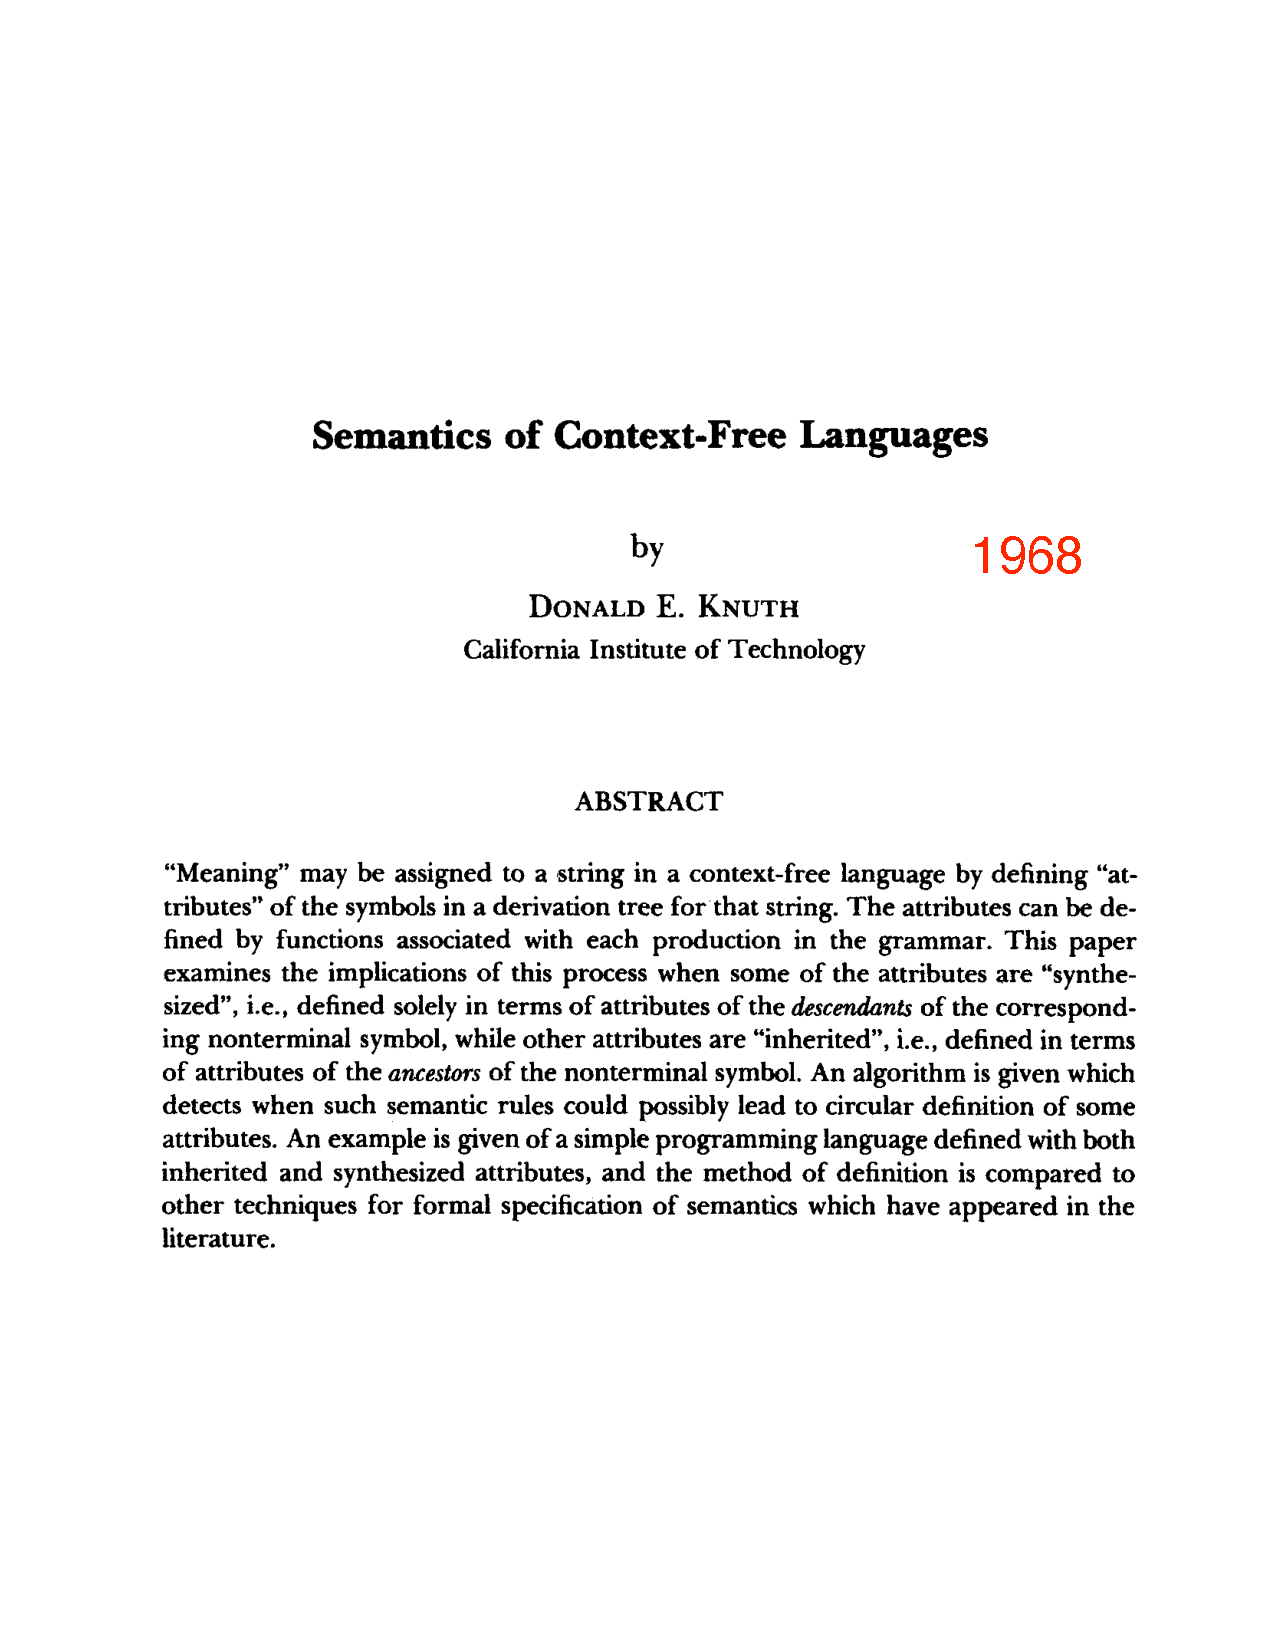
\includegraphics[width=0.95\linewidth,trim={0 0 0 7cm},clip]{Knuth-Page-1-with-date.pdf}
\end{frame}
\note{\bi
\x Knuth had his hands in everything ...
\x errors in the original paper, so he's not perfect
\x not a universally loved formalism, seen as ``academic''
\ei
}


\begin{frame}{After all these years, why attribute grammars?}
\pause
Motivated by 4 questions

\bigskip\pause
\bes{0.3cm}
\x Can programming languages be constructed from composable modules, \\
   each defining an extension to a host language?

\pause
\x Can extensions add new syntax and new static semantics?

\pause
\x Can extension be developed independently?

\pause
\x Can programmers compose the extensions of their choosing \\
   \underline{without} needing to understand the underlying
   implementations?

   \bigskip
   Distinguish the roles of extension developer and extension user
   (the programmer).

   \pause
   \bigskip
   For example, can one add \hir{Cilk-style parallelism}, \hib{algebraic data types},
   and \hig{regular expressions} to C?
\ee

\note{\bi
\x Traditional reasons: language prototyping, tool generation
\x My reasons: modularity and composability
\ei
}
\end{frame}

\newcommand{\rx}[1]{\textcolor{LimeGreen}{#1}}
\newcommand{\adt}[1]{{\usebeamercolor[fg]{bluecolor}#1}}

\newcommand{\cilk}[1]{\hir{#1}}
\newcommand{\regex}[1]{\hig{#1}}

\begin{frame}[t,fragile]
\small
\begin{alltt}
\begin{tabbing}
aa\=aa\=aa\=aa\=aa\=aa\=\kill
typedef \hib{datatype Tree} Tree; \\

\hib{datatype Tree \ttlbrace} \\
\>\hib{Fork (} Tree*\hib{,} Tree*\hib{,} const char* \hib{);} \\
\>\hib{Leaf (} const char* \hib{); }\\
\hib{\ttrbrace;} \\
\\

\cilk{cilk} int count_matches (Tree *t) \ttlbrace \\
  \hib{match (} t \hib{) \ttlbrace} \\
    \hib{Fork(t1, t2, str): \ttlbrace} \\ 
      int res_t, res_t1, res_t2;   \\
      \cilk{spawn res_t1 = count_matches(} t1 \cilk{);}  \\
      \cilk{spawn res_t2 = count_matches(} t2 \cilk{);}  \\
      res_t = ( str \regex{=~ /foo[1-9]+/} ) ? 1 : 0;  \\
      \cilk{sync;} \\
      \cilk{cilk return} res_t1 + res_t2 + res_t \cilk{;} \\
    \hib{\ttrbrace ;}  \\
    \hib{Leaf(str): \ttlbrace} return ( str \regex{=~ /foo[1-9]+/} ) ? 1 : 0; \hib{\ttrbrace ;} \\
  \hib{\ttrbrace}  \\
\ttrbrace
\end{tabbing}
\end{alltt}
\end{frame}


\begin{comment}
\begin{frame}{A demonstration}

\ableC{} - Attribute grammar-Based Language Extensions for C

\note{\bi
\x In \code{/Users/evw/ableC\_Demo}
\x Parallel Tree Search - pts.xc
 \bi
  \x show in Atom in ``demo'' mode
  \x turn off demo mode
 \ei
\x compiler and run it.
\x Syntax
\x Cilk - creates two clones for each function 
 \bi
  \x thus traverses the AST, even other extension components
 \ei

\ei
}
\end{frame}
\end{comment}


\begin{frame}[fragile]{\ableC - extensible specification of C11}

\begin{minipage}[c]{2.1in}
\begin{center}

\vskip 0.1cm

\uncover<1->{\exts{org:fp:algebraicDataTypes}} \\
\uncover<1->{\exts{com:parallel:cilk}} \\
\uncover<1->{\exts{net:foo:regEx}}

\uncover<2->{
$\Downarrow$

\ewhite{$\Longrightarrow$ $\Longrightarrow$}
\framebox{\texttt{Silver}}  
$\Longrightarrow$ $\Longrightarrow$ 

$\Uparrow$}

\uncover<1->{\exts{edu:umn:cs:melt:ableC}}

\verb!  !

\verb!  !

\end{center}
\end{minipage}
\begin{minipage}[c]{1.15in}
\begin{center}

%\vskip 0.2cm

\uncover<3->{\tcode{pts.xc}}

\uncover<4->{$\Downarrow$}

\uncover<4->{\framebox{\texttt{cpp}}}

\uncover<4->{$\Downarrow$}

\uncover<4->{\tcode{pts.i}}

\uncover<5->{$\Downarrow$}

\uncover<2->{\framebox{\texttt{ableC.jar}}}

\uncover<5->{$\Downarrow$}

\uncover<5->{\tcode{pts.c}}

\uncover<6->{$\Downarrow$}

\uncover<6->{\framebox{\texttt{gcc}}}

\uncover<6->{$\Downarrow$}

\uncover<6->{\tcode{a.out}}
\end{center}
\end{minipage}
\begin{minipage}[c]{0.5in}
\vskip 0.1cm
\uncover<7->{
\begin{equation*}
\begin{cases}
- scanning \\
- parsing \\
- AST\ construction\\
- type\ checking\\
- optimization\\
- C\ code \ generation
\end{cases}
\end{equation*}
}
\end{minipage}

\note{\bi
\x After the demo - show this slide.
\ei
}
\end{frame}







\begin{frame}{Reliably composable language extensions}
\biA
\x Extension \hib{developers} work independently.

\x Extension \hib{users} use multiple extensions.
 \bi
  \x not experts in language design
  \x combinations of extensions must ``just work''
 \ei
\x We draw a hard distinction between these two roles.
\ei
\note{\bi
\x We \hib{distinguish these two roles}!
\ei
}
\end{frame}

\begin{frame}[t]{Challenges for composable language extensions}
%Two primary challenges:
\be
 \x syntax ---     context free grammars / regular expressions

    need a deterministic parser and scanner

  \bi
   \x<2-> context-aware scanning %~\cite{vanwyk07gpce}
   \x<4-> \hib{modular determinism analysis} %~\cite{schwerdfeger09pldi} 
   \x<5-> Copper
  \ei
%\vskip 0.5cm
 \x static semantics ---     attribute grammars
    
    need complete static analysis and translations

  \bi
   \x<3-> forwarding % - solves the ``expression problem''
   \x<3-> set union of specification components
    \bi
     \x sets of productions, non-terminals, attributes
     \x sets of attribute defining equations, on a production
     \x sets of equations contributing values to a single attribute
    \ei
   \x<4-> \hib{modular well-definedness analysis} %~\cite{kaminski12sle}
%   \x<5-> modular termination analysis %~\cite{krishnan12sle,krishnan12phd}
   \x<5-> Silver
  \ei
\ee

\end{frame}



\begin{frame}[t,fragile]{Representing Programs}
Consider a let-expressions language: 
``\code{let n = true in false || n}''

\bigskip

\begin{minipage}[t]{2.9in}
\vspace{0pt}
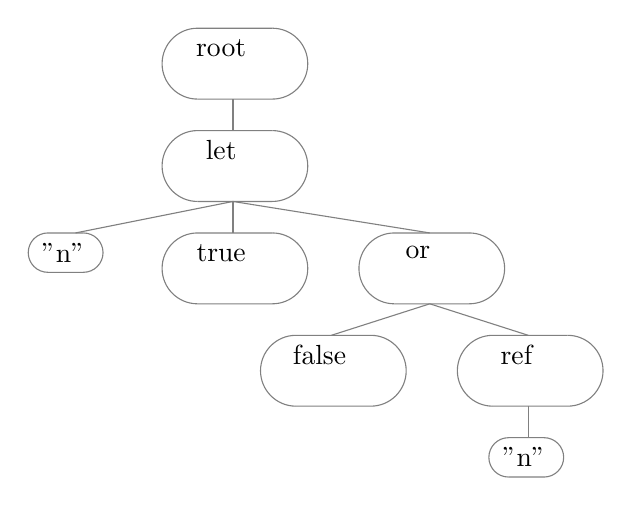
\begin{tikzpicture}

%\draw ($(5.5,\ys*-0.5)$) node {\small\texttt{body.env = addEnv(name, dval.val, e.env);}};

% env on the side
%\envc{1.8}{4}
%\draw (1.9,4.85) node{env};

%\ppc{1}{3.5}
%\draw (1.84,4.18) node{pp};

%\valc{0.6}{3}
%\draw (1.88,3.6) node{val};

\rtnna{4}{4}{root}
\tedge{4}{4}{4}{3}

\tnna{4}{3}{let}
\tedge{4}{3}{2.0}{2}
\tedge{4}{3}{4}{2}
\tedge{4}{3}{6.5}{2}

\tnstr{2.0}{2}{"n"}

\tnna{4}{2}{true}

\tnna{6.5}{2}{or}
\tedge{6.5}{2}{5.25}{1}
\tedge{6.5}{2}{7.75}{1}

\tnna{5.25}{1}{false}

\tnna{7.75}{1}{ref}
\tedge{7.75}{1}{7.75}{0}

\tnstr{7.85}{0}{"n"}

%\ppeval

%\valeval
\end{tikzpicture}
\end{minipage}
\begin{minipage}[t]{2.1in}
\vspace{0pt}
\small
\begin{verbatim}
nonterminal Root, Expr;

production root
 r::Root ::= e::Expr

production let
 e::Expr ::= name::String 
    dexp::Expr body::Expr

production or
 e::Expr ::= l::Expr r::Expr

production ref
 e::Expr := name::String
\end{verbatim}
\end{minipage}

\end{frame}




\begin{frame}[t,fragile]{Attributes: attaching semantic values}
Can we pretty-print and evaluate the expression
``\code{let n = true in false || n}'' ?

\bigskip

\begin{minipage}[t]{2.9in}
\vspace{0pt}
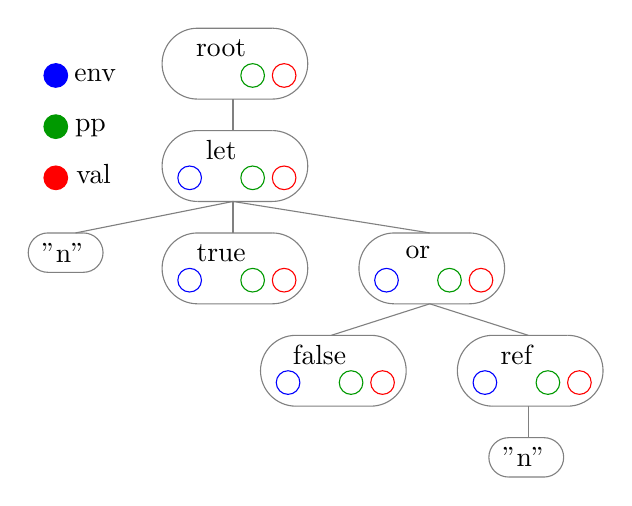
\begin{tikzpicture}

%\draw ($(5.5,\ys*-0.5)$) node {\small\texttt{body.env = addEnv(name, dval.val, e.env);}};

% env on the side
\envc{2.3}{4}
\draw (2.4,4.85) node{env};

\ppc{1.5}{3.5}
\draw (2.34,4.18) node{pp};

\valc{1.1}{3}
\draw (2.38,3.6) node{val};

\rtn{4}{4}{root}
\tedge{4}{4}{4}{3}

\tn{4}{3}{let}
\tedge{4}{3}{2.0}{2}
\tedge{4}{3}{4}{2}
\tedge{4}{3}{6.5}{2}

\tnstr{2.0}{2}{"n"}

\tn{4}{2}{true}

\tn{6.5}{2}{or}
\tedge{6.5}{2}{5.25}{1}
\tedge{6.5}{2}{7.75}{1}

\tn{5.25}{1}{false}

\tn{7.75}{1}{ref}
\tedge{7.75}{1}{7.75}{0}

\tnstr{7.85}{0}{"n"}

%\ppeval

%\valeval
\end{tikzpicture}
\end{minipage}
\begin{minipage}[t]{2.1in}
\vspace{0pt}
\small
\begin{verbatim}
synthesized attribute pp::String;

synthesized attribute val::Boolean;

inherited attribute 
  env::[(String,Boolean)];


attribute pp  occurs on Root, Expr;

attribute val occurs on Root, Expr;

attribute env occurs on Expr;
\end{verbatim}
\end{minipage}

\end{frame}

\begin{frame}{Equations}
Let's look at some Silver specifications for this.

\bigskip
See \code{AbstractSyntax.sv}
\end{frame}


\begin{frame}[t,fragile]{Evaluating attributes}
Demand \code{pp}, then demand \code{val} in ``\code{let n = true in false || n}''

\bigskip

\begin{minipage}[t]{2.9in}
\vspace{0pt}
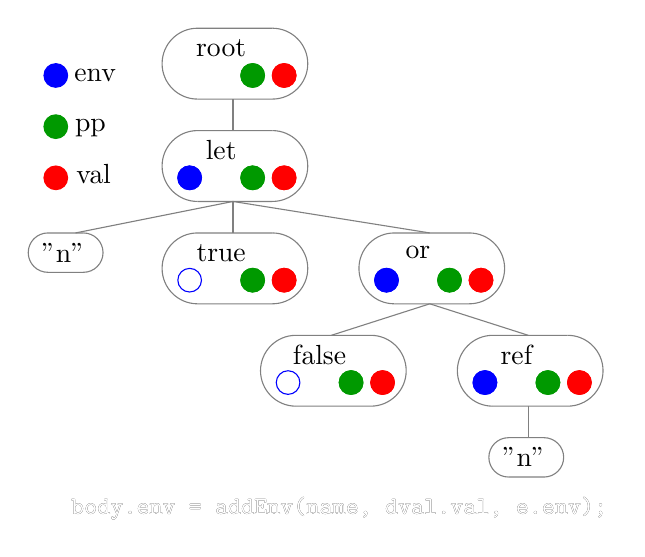
\begin{tikzpicture}

%\draw ($(5.5,\ys*-0.5)$) node {\small\texttt{body.env = addEnv(name, dval.val, e.env);}};

\envc{2.3}{4}
\draw (2.4,4.85) node{env};

\ppc{1.5}{3.5}
\draw (2.34,4.18) node{pp};

\valc{1.1}{3}
\draw (2.38,3.6) node{val};

\rtn{4}{4}{root}
\tedge{4}{4}{4}{3}

\tn{4}{3}{let}
\tedge{4}{3}{2.0}{2}
\tedge{4}{3}{4}{2}
\tedge{4}{3}{6.5}{2}

\tnstr{2.0}{2}{"n"}

\tn{4}{2}{true}

\tn{6.5}{2}{or}
\tedge{6.5}{2}{5.25}{1}
\tedge{6.5}{2}{7.75}{1}

\tn{5.25}{1}{false}

\tn{7.75}{1}{ref}
\tedge{7.75}{1}{7.75}{0}

\tnstr{7.85}{0}{"n"}

\ppeval

\valeval
\end{tikzpicture}
\end{minipage}
\begin{minipage}[t]{2.1in}
\vspace{0pt}

\end{minipage}
\end{frame}


\begin{frame}{Higher order attributes}
\biA
 \x Synthesized and inherited attributes can be \hib{syntax trees}.

 \x Such a tree can be ``rooted'' so that
  \bi
   \x by giving it inherited attributes
   \x synthesized attributes can be computed and accessed.
  \ei

 \x \code{synthesized attribute inline :: Expr occurs on Expr;}

    \medskip
    A program transformation to inline the identifies.

 \x We see this in \code{Inline.sv}
\ei
\end{frame}

\begin{frame}{Automatic attributes}
\biA
 \x Many equations follow a predictable pattern can be generated to
 \hib{propagate} values in the expected way.

 \x For inherited attributes - just copy them down the tree

 \x For rewriting attributes - recreate the node with the rewritten
 children

 \x \code{propagate} performs this generation
 \x \code{inherited}, \code{functor} attributes and others can then
 have equations generated

 \x See \code{Inline.sv} again.
\ei
\end{frame}

\begin{frame}{Reference attributes}
\bis{0.3cm}
\x These are ``references'' to remote decorated tree nodes.

   \medskip
   We can access attributes from references, just as on child nodes.

\pause
\x We saw 2 environments to provide
  \be
   \x the value and 
   \x the inlined expression
  \ee
  for name uses.

\x Can we instead map names to a tree node describing the declaration which
   may have this information.

   \medskip
   What kind of tree node should be the target?

   \medskip
   Not \code{Expr}, a bit of refactoring is needed to create a
   declaration node type \code{Decl}.

\x \code{inherited attribute env :: [ (String, Decorated Decl) ];}

\x This requires a bit of refactoring - \code{Inline\_Refs.sv}
\ei
\end{frame}


\begin{frame}{Language Extensions}
\biA
\x Refactor inlining out into an extension
\x Create the \code{implies} production in another extension
\x How does implies know about inlining?
\x This motivates forwarding
\ei
\end{frame}

% mv Main.sv into composed


\begin{frame}[fragile,t]{Forwarding}
``no glue code'' for extensions

{\small
\begin{verbatim}
production implies
e::Expr ::=  l::Expr  r::Expr
{ e.pp = "(" ++ l.pp ++ "=>" ++ r.pp ++ ")";
  forwards to or( not(l), r ); {- expr, not template -}  }
\end{verbatim}
}

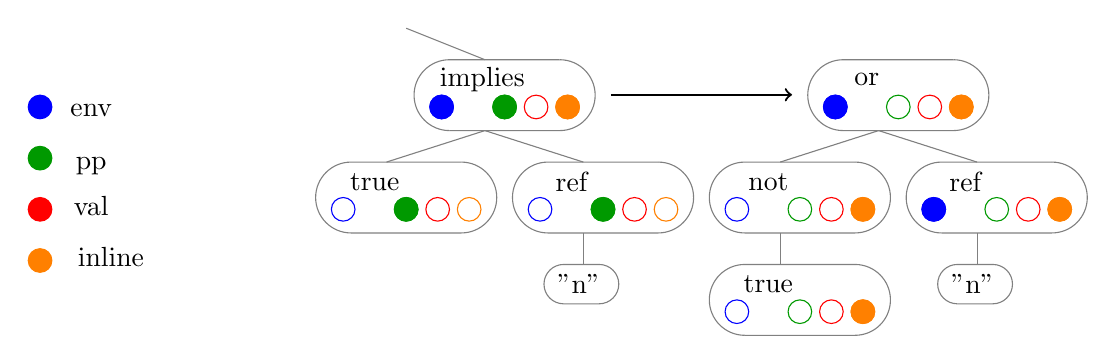
\begin{tikzpicture}
\showimplies
\end{tikzpicture}

\end{frame}


\begin{frame}[t]{Modular Well-definedness Analysis}
How can we ensure that independent extensions will compose?

\medskip
How can we ensure that there are no missing equations in the
composition by looking at the extensions individually?

\bigskip

$\mathit{complete} ( H \cup \{ E_1, ... , E_n \} ) $ \ \ ?

%\pause
\bigskip

$\forall i \in [1,n] . \mathit{modComplete}(H, E_i) 
 \Rightarrow \mathit{complete}( H \cup \{ E_1, ..., E_n \} )$

\bigskip
In three parts:
\be
 \x well-formedness
 \x synthesized completeness
 \x effective inherited completeness
\ee
\end{frame}


\begin{frame}

ending slides
\end{frame}


\end{document}

\begin{frame}{Table of Contents}
\bi
\x ASTs - how we represent a program
\bi
\x \code{let n = true in false || n},  show the tree
\x show the context free grammar - nonterminals and productions
\x slides 35 and previous in other talk
\ei
\x AGs - how we type check, analyze, and translate that program
\bi
\x attributes decorate nodes
\x show tree with the dots all filled in - think of these as records
\x fill in AG with attributes A and occurs on relation 

\x equations specify their value

\x new analysis/transformation - inlining

\x higher order - maybe a translation to something - a stack machine
for evaluation

\x new productions - 
\x reference attributes

\x forwarding

\x MWDA
\ei
\ei
\end{frame}



% 999 
\eedd

\begin{comment}
\begin{frame}{Welcome - RM}

Today we will discuss and use the \ableC{} extensible language
framework.  

\bigskip
Language extensions can be developed independently to
target different problem domains.  

\bigskip
Certain composability criteria
ensure that different extensions can be composed to form a working
compiler.  

\bigskip
These criteria are checked on extensions independently of
others. 
\end{frame}

\begin{frame}{Today - RM}
\bi
\x \ableC{} - an extensible specification of C11
\x use \ableC{} from a programmers perspective
\x develop and modify language extensions to
 \bi
  \x add new concrete syntax / notations
  \x define their abstract syntax and translation to plain C
  \x perform type checking
  \x implement simple optimizations
  \x understand scanning, parsing, and attribute grammars
 \ei
\x use modular composability analyses to check for composability
\ei
\end{frame}
\end{comment}


\newcommand{\cwidth}{9}
\newcommand{\cheight}{6.75}

\newcommand{\showaxes}[1]{
\draw[step=.5,white,very thin] (0,0) grid ($(\cwidth,\cheight+1)$);

% axes
\draw[->,thick] (0,0) -- (\cwidth,0);
\draw[->,thick] (0,0) -- ($(0,\cheight-0.5)$);

% labels
\draw[left] ($(-0.3,\cwidth*0.5)$) node[rotate=90,]{variants};
\draw ($(\cheight*0.5,-0.3)$) node{operations};

% origin
%\filldraw[gray] (0,0) circle (\cwidth*0.02);
%\draw[<-] (0.25,0.25) arc (160:100:0.5);
%\draw (0.9,0.6) node{$\emptyset$};

% base type
\filldraw[gray] ($(\cwidth*0.3,\cheight*0.3)$) circle (\cwidth*0.02);
\draw[->] ($(\cwidth*0.3-0.5,\cheight*0.3-0.7)$) arc (280:350:0.5);
\draw[right] ($(\cwidth*0.3-1.5,\cheight*0.3-0.7)$) node{#1};

}

\newcommand{\oopfp}{
\draw[->,blue,very thick] ($(\cwidth*0.3+0.25,\cheight*0.3)$) -- 
               ($(\cwidth-1,\cheight*0.3)$);

\draw[->,blue, very thick] ($(\cwidth*0.3,\cheight*0.3+0.25)$) -- 
               ($(\cwidth*0.3,\cheight-1.0)$);

\draw ($(\cwidth*0.6,\cheight*0.3-0.3)$) node{FP - new functions}; 

\draw ($(\cwidth*0.3-1.2,\cheight*0.6)$) 
  node[text width=2cm, align=center]{OOP -  new subclasses}; 
}

\newcommand{\oopfpprobs}{

% extended type
\filldraw[gray] ($(\cwidth*0.6,\cheight*0.6)$) circle (\cwidth*0.02);
\draw[->] ($(\cwidth*0.6-0.5,\cheight*0.6-0.7)$) arc (280:350:0.5);
\draw[right] ($(\cwidth*0.6-2.3,\cheight*0.6-0.7)$) node{extension};

\pause
% OOP challenges
\draw[<-,red]
   ($(\cwidth*0.6,\cheight*0.6+0.5)$) --
   ($(\cwidth*0.6,\cheight*0.6+1.25)$) ;

\draw 
   ($(\cwidth*0.6,\cheight*0.6+2.25)$) 
   node[text width=3cm, align=center]{OOP - modify classes to add methods}; 


% FP challenges
\draw[<-,red] ($(\cwidth*0.6+0.5,\cheight*0.6)$) --
          ($(\cwidth*0.6+1.25,\cheight*0.6)$) ;
\draw     ($(\cwidth*0.6+2.25,\cheight*0.6)$) 
  node[text width=2cm, align=center]{FP - modify functions to add clauses}; 
}


\begin{frame}[t]{Extensible Languages}
Base = Host Programming Language

\bi
 \x new variants = new (abstract) syntax

 \x new operations = new semantic analysis, translations
\ei

\begin{tikzpicture}[scale=0.85, every node/.style={scale=0.85}]
\draw[step=.5,white,very thin] (0,0) grid ($(\cwidth,\cheight)$);

% axes
\draw[->,thick] (0,0) -- (\cwidth,0);
\draw[->,thick] (0,0) -- ($(0,\cheight-0.5)$);

% labels
\draw[left] ($(-0.3,\cwidth*0.5)$) node[rotate=90,]{syntax};
\draw ($(\cheight*0.5,-0.3)$) node{semantic analysis, translations};

% origin
%\filldraw[gray] (0,0) circle (\cwidth*0.02);
%\draw[<-] (0.25,0.25) arc (160:100:0.5);
%\draw (0.9,0.6) node{$\emptyset$};

% base type
\filldraw[gray] ($(\cwidth*0.3,\cheight*0.3)$) circle (\cwidth*0.02);
\draw[->] ($(\cwidth*0.3-0.5,\cheight*0.3-0.7)$) arc (280:350:0.5);
\draw[right] ($(\cwidth*0.3-1.5,\cheight*0.3-0.7)$) node{\ \ C};




\filldraw[gray] ($(\cwidth*0.6,\cheight*0.6)$) circle (\cwidth*0.02);
\draw[->] ($(\cwidth*0.6-0.5,\cheight*0.6-0.7)$) arc (280:350:0.5);
\draw[right] ($(\cwidth*0.6-2.6,\cheight*0.6-0.7)$) node{extended C};

\draw
   ($(\cwidth*0.6+3.7,\cheight*0.6+0.15)$) 
   node[text width=8cm, align=left]
     {\bi \x[] inductive datatypes extension
          \x[] regex matching extension
          \x[] parallel programming extension
      \ei};

\end{tikzpicture}
\end{frame}


%\begin{comment}
\begin{frame}{Directions of Extensibility}

\begin{tikzpicture}[scale=0.95, every node/.style={scale=0.95}]
\showaxes{base}
\pause
\oopfp{}
\pause
\oopfpprobs{}
\end{tikzpicture}

\end{frame}


\begin{frame}[t]{The Expression Problem}
Requirements for solving it:
\be
 \x extensibility in both directions
 \x strong static typing
 \x no modification of existing code
 \x separate compilation and type checking
\ee

\bigskip
Old problem, new name popularized by Phil Wadler.

\bigskip
Allows
\be
 \x a linear ordering of extensions

    $Base \triangleleft E_1 \triangleleft E_2$

 \x $E_2$ developer writes code to handle $E_1$
\ee
\end{frame}


\begin{frame}[t]{Independently extensible version}
Requirements for solving it:
\be
 \x \egray{extensibility in both directions}
 \x \egray{strong static typing}
 \x \egray{no modification of existing code}
 \x \egray{separate compilation and type checking}
 \uncover<2->{\x no linear ordering of extensions

   $Base \triangleleft E_1 \triangleleft E_2$

   $Base \triangleleft E_2 \triangleleft E_1$}
\ee

\uncover<3->{
\medskip
Zenger and Odersky

\medskip
Allows
\be
 \x ``glue'' code to compose extensions

    written by $3^{rd}$ party to compose $E_1$ and $E_2$

    \eg\ the operation in $E_1$ for variant in $E_2$
\ee
}
\note{
\bi
 \x Show \code{pts.xc} again
 \x It would not be the programmer that just ``imports'' extensions
 \x They may need to write some AG specs.
 \x We don't want that.
\ei
}
\end{frame}


\begin{comment}
\newcommand{\cilk}[1]{\hir{#1}}
\newcommand{\regex}[1]{\hig{#1}}

\begin{frame}[t,fragile]
\small
\begin{alltt}
\begin{tabbing}
aa\=aa\=aa\=aa\=aa\=aa\=\kill
typedef \hib{datatype Tree} Tree; \\

\hib{datatype Tree \ttlbrace} \\
\>\hib{Fork (} Tree*\hib{,} Tree*\hib{,} const char* \hib{);} \\
\>\hib{Leaf (} const char* \hib{); }\\
\hib{\ttrbrace;} \\
\\

\cilk{cilk} int count_matches (Tree *t) \ttlbrace \\
  \hib{match (} t \hib{) \ttlbrace} \\
    \hib{Fork(t1,t2,str): \ttlbrace} \\ 
      int res_t, res_t1, res_t2;   \\
      \cilk{spawn res_t1 = count_matches(} t1 \cilk{);}  \\
      \cilk{spawn res_t2 = count_matches(} t2 \cilk{);}  \\
      res_t = ( str \regex{=~ /foo[1-9]+/} ) ? 1 : 0;  \\
      \cilk{sync;} \\
      \cilk{cilk return} res_t1 + res_t2 + res_t \cilk{;} \\
    \hib{\ttrbrace ;}  \\
    \hib{Leaf(str): \ttlbrace} return ( str \regex{=~ /foo[1-9]+/} ) ? 1 : 0; \hib{\ttrbrace ;} \\
  \hib{\ttrbrace}  \\
\ttrbrace
\end{tabbing}
\end{alltt}
\end{frame}
\end{comment}
%\hib{match (str) (} \\ 
%                          \regex{/bar[1-9]+/} \hib{:} 1 \hib{;}  \\
%                          \hib{_ :} 0 \hib{;} \\
%                        \hib{) ; \ttrbrace} \\


\newcommand{\them}[1]{\hib{#1}}
\newcommand{\us}[1]{\hir{#1}}


\begin{frame}[t]{Another Expression Problem}
Requirements for solving it:
\be
 \x \egray{extensibility in both directions}
    \hfill \uncover<4->{\them{Attribute grammars}}
 \x \egray{strong static typing}
    \hfill \uncover<5->{\us{Effective completeness analysis}}
 \x \egray{no modification of existing code}
    \hfill \uncover<4->{\them{Attribute grammars}}
 \x \egray{separate compilation and type checking}
    \hfill \uncover<5->{\us{Modular effective completeness analysis}}
 \x \egray{no linear ordering of extensions
     \hfill \uncover<4->{\them{Attribute grammars}}

   $Host \triangleleft E_1 \triangleleft E_2$

   $Host \triangleleft E_2 \triangleleft E_1$}

 \x<2-> no glue code, composition is automatic
    \uncover<5->{\hfill \us{Forwarding}}
\ee

\bigskip
\uncover<3->{Allows
\bi
 \x a non-expert programmer to do the composition
\ei

But it requires
\bi
 \x extensions are somehow realizable in the base
 %\x extension language constructs translate down to host language constructs
\ei
}
\end{frame}




\begin{comment}
\begin{frame}{An analogy}
\biA
\x We \hib{can} write type safe programs in assembly, Python, Ruby, Scheme,
etc.
\pause
\x We \hig{are guaranteed to} write type safe program in ML, Haskell,
etc.
\x Some of us (happily) trade some expressibility for this safety.
\pause
\x \hib{Can} we build extensible languages and composable language extensions?
\pause
\x Are there any \hig{guarantees} of composability of language extensions?
\ei
\end{frame}
\end{comment}

\begin{frame}{A detour - for concrete syntax}

\includegraphics[width=0.7\linewidth]{detour.jpg}

\end{frame}


% ----------------------------------------------------------------------
\section{Concrete Syntax}

 

\begin{frame}{Parsing composed languages}

Can we build a deterministic (non-ambiguous) parser from composed
specifications? 

\vskip 0.25cm
\bis{0.3cm}
 \x {\large $CFG_C = CFG^H \cup^* \{ CFG^{E_1}, ... , CFG^{E_n} \}$}

 \x Monolithic analysis of $CFG_C$ is too hard, but not useful.

 \pause

 \x A \hib{modular} analysis is required %~\cite{schwerdfeger09pldi}.

 \x 
{\large
\begin{tabbing}
  \only<2->{$\forall i \in [1,n]\ .$}\ \= 
    \only<2>{\ \ \ $?$}
    \only<3->{$\mathit{isComposable}(CFG^H, CFG^{E_i})\ \ \ \land$} \\
 \>  \only<3->{$\mathit{conflictFree}(CFG^H \cup CFG^{E_i})$}  \\

 \only<2->{$\Rightarrow \mathit{conflictFree}(CFG^H \cup \{ CFG^{E_1},
   ... , CFG^{E_n} \})$} 
\end{tabbing}
}


\x<3-> \hib{Non-commutative} composition of restricted LALR(1) grammars.
\x<3-> \eblue{isComposable} is an analysis that the language extension
          designer can run. 
%\bi
% \x It certifies individual grammars with respect to a host language.
% \x All certified extension grammars can be be composed - to form a
%    deterministic grammar.
%\ei
\ei
\end{frame}


\begin{frame}{Challenges in scanning}
A better scanner enables this modular analysis.

\pause
\bis{0.25cm}

\x Keywords in embedded languages may be identifiers in host language:

\begin{tabbing}
\codesblue{int \codesblack{SELECT} ;} \\
\codesblue{...} \\
\codesblue{rs = using c query \{ }\=\codesblue{\codesblack{SELECT} last\_name}  \\
\>\codesblue{FROM person WHERE ... } 
\end{tabbing}
\pause

\x Different extensions use same keyword

\begin{tabbing}
\codesblue{conn}\=\codesblue{ection c "jdbc:derby:./derby/db/testdb"} \\
\>\codesblue{with \codesblack{table} person [ }\=\codesblue{person\_id INTEGER,} \\
\>\>\codesblue{first\_name VARCHAR ];} \\
\codesblue{...}\\
\codesblue{b = \codesblack{table} ( }\=\codesblue{c1 :  T F ,}\\
\>\codesblue{c2 :  F * ) ;}
\end{tabbing}
\ei
\end{frame}


\begin{frame}{Challenges in scanning}
\bis{0.3cm}

\x Operators with different precedence specifications:

\codesblue{
\begin{tabbing}
x = 3 + y \codesblack{*} z ; \\
...\\
str =\tttilde{} /[a-z][a-z0-9]\codesblack{*}$\backslash$.java/
\end{tabbing}}
\pause

\x Terminals that are prefixes of others

\codesblue{
\begin{tabbing}
List<List<Integer\codesblack{>>} dlist ; \\
...\\
x = y \codesblack{>>} 4 ; 
\end{tabbing}}
\pause
or
\codesblue{
\begin{tabbing}
aspect ... before ... call( o.\codesblack{get*}() ) \\
... \\
x = \codesblack{get*}3 ; 
\end{tabbing}}
\scriptsize{[from Bravenboer, Tanter \& Visser's OOPSLA 06 paper on parsing AspectJ]}
\ei
\end{frame}

%Distinguish 
% - terminal names
% - terminal literals
% - nonterminal names

% - extension versus host


\begin{frame}{Need for context}
\bis{0.25cm}
\x \hir{Problem:} the scanner cannot match strings (lexemes) to
proper terminal symbols in the grammar.  

\begin{tabbing}
MMMMMMM\=MMMMMMMMMMMM\=MMM\=\kill
``\texttt{SELECT}'' \>-- \term{Select} \> or \> \term{Id} \\
``\texttt{table}''  \>-- \term{SQL\_table}  \> or \> \term{DNF\_table} \\
``\texttt{>>}''     \>-- \term{RightBitShift}   \> or \>   \term{GT},  \term{GT}
\end{tabbing}
\pause
\x Neither terminal has global precedence over the other. 
\bi \x maximal munch gives ``\code{>>}'' precedence over ``\code{>}''
    \x thus grammars are written to accommodate this
\ei

\x If the scanner can distinguish between them, the context free
   grammar can be simplified:
\bi 
 \x \nt{typeExpr} $::=$  \term{Id}\ $|$ \ \term{Id}  \termlit{<}
    \nt{typeExpr} \termlit{>}
 \ei
\ei
\end{frame}


\begin{frame}{Need for context}
\bi
\x % Problem is scanner is unaware of the context.
Traditionally, parser and scanner are disjoint.

\vskip 0.75cm

$\framebox{Scanner} \rightarrow \framebox{Parser}
\rightarrow \framebox{Semantic Analysis}$

\vskip 0.75cm

\x In context aware scanning, they communicate

\vskip 0.75cm

$\framebox{Scanner}\ \ered{\rightleftarrows}\ \framebox{Parser}
\rightarrow \framebox{Semantic Analysis}$

\ei
\end{frame}


\begin{frame}{Context aware scanning}
\bis{0.4cm}
\x We use a slightly modified LR parser and a context-aware scanner.
\x Context is based on the LR-parser state.
\x \eblue{Parser passes a set of valid look-ahead terminals to
  scanner.}
\x This is the set of terminals with \emph{shift}, \emph{reduce}, or
\emph{accept} entries in parse table for current parse state. 

\pause
\x \eblue{Scanner only returns tokens from the valid look-ahead set.}
\x Scanner uses this set to \eorange{disambiguate} terminals. 


\begin{tabbing}
MMMMMMM\=MMMMMMMMMMMM\=MMM\=\kill
``\texttt{SELECT}'' \>-- \term{Select} \> or \> \term{Id} \\
``\texttt{table}''  \>-- \term{SQL\_table}  \> or \> \term{DNF\_table}  \\
``\texttt{>>}''     \>-- \term{RightBitShift}   \> or \>   \term{GT},  \term{GT}
\end{tabbing}

%\bi
% \x \eg{} \term{SQL\_table}  \ or \ \term{DNF\_table} 
% \x \eg{} \term{Select} \ \ \ \ \ \ \ or \ \term{Id} 
%\ei
\ei
\end{frame}


\begin{frame}{Context aware scanning}
\biA
\x \eblue{This scanning algorithm subordinates the principle of} \\ 
   \egreen{disambiguation by maximal munch}  \\
   \eblue{to the principle of}  \\
   \egreen{disambiguation by context.}
\pause
\x It will return a shorter valid match before a longer invalid match.

\x Before ``\eblue{\texttt{>}}'' in \eblue{\texttt{List<List<Integer>>}}, 
``\eblue{\texttt{>}}'' in valid look-ahead but  ``\eblue{\texttt{>>}}'' is not. 

   (This example does not actually work in Java.)

\x A context aware scanner is essentially an implicitly-moded scanner.

   Each parse state represents a different mode.

\x There is no explicit specification of valid look ahead.  
   \bi \x It is generated from standard grammars and terminal regexs.
   \ei
\ei
\end{frame}


\begin{frame}{Lexical Precedence}
\biA
 \x A notion of lexical precedence is still needed, \eg\ to prefer
    keywords to identifiers.
\pause
 \x This precedence is global
  \biA
   \x \term{While}  $>$  \term{Id}
   \x in all contexts, ``\texttt{while}'' is scanned as \term{While},
      not a \term{Id},
   \x even contexts that contain \term{Id} but not \term{While}
   \x \eg\ in ``\texttt{if while then}'' - see ``\texttt{while}'' as
   \term{While} even though it is not in valid look-ahead set as computed
   by parser. 
  \ei
%e.g. Select_kwd > SQL_Identifier
%Select_kwd and Identifier not in same valid lookahead set.
%In SQL contexts we prefer Select_kwd over SQL_Ids.
%In these contexts, Identifier is not in valid lookahead set.

%\x Some examples will help clarify...
\ei
\note{Go fast, skip details, this is not interesting.}
\end{frame}


\newcommand{\bcode}[1]{\scriptsize{\texttt{#1}}}

\newcommand{\lineh}{0.35}
\newcommand{\colw}{0.149}
\newcommand{\lineoffset}{1.1}
\newcommand{\coloffset}{0.4}

\newcommand{\pointer}[3]{%
\only<#1>{\draw[->,ultra thick,blue]
  ($(\colw*#2+\coloffset,\lineh*#3+\lineoffset)$) arc (150:180:2);}}

\newcommand{\pntr}[2]{\draw[->,ultra thick,blue]
  ($(\colw*#1+\coloffset,\lineh*#2+\lineoffset)$) arc (150:180:2);}

\newcommand{\validla}[1]{\draw[right] (6,8.3) node {Valid look-ahead set:}
                                      (6,7.8) node {\{ #1, ... \}}; }
\newcommand{\validlatwo}[2]{\draw[right] (6,8.3) node {Valid look-ahead set:}
                                         (6,7.8) node {\{ #1}
                                         (6.35,7.3) node {#2, ... \}}; }

\newcommand{\dspvalid}[4]{\only<#1>{\pntr{#2}{#3}}\only<#1>{\validla{#4}}}
\newcommand{\dspvalidtwo}[5]{\only<#1>{\pntr{#2}{#3}}\only<#1>{\validlatwo{#4}{#5}}}


\newcommand{\showcode}{\draw[right]
 ($(\colw*0,\lineh*24)$) node {\bcode{class Demo \{}} 
 ($(\colw*2,\lineh*23)$) node {\bcode{int demoMethod ( ) \{}} 
 ($(\colw*4,\lineh*22)$) node {\bcode{List<List<Integer>> dlist ;}} 
 ($(\colw*4,\lineh*21)$) node {\bcode{int T ;}} 
 ($(\colw*4,\lineh*20)$) node {\bcode{int SELECT ;}} ;
\draw[right, blue]
 ($(\colw*4,\lineh*19)$) node {\bcode{connection c "jdbc:derby:/home/derby/db/testdb"}} 
 ($(\colw*6,\lineh*18)$) node {\bcode{with table person [ person\_id INTEGER, }} 
 ($(\colw*26,\lineh*17)$) node {\bcode{first\_name VARCHAR,}} 
 ($(\colw*26,\lineh*16)$) node {\bcode{last\_name VARCHAR ] ,}} 
 ($(\colw*11,\lineh*15)$) node {\bcode{table details [ person\_id INTEGER,}} 
 ($(\colw*27,\lineh*14)$) node {\bcode{age INTEGER ] ;}} ;
\draw[right]
 ($(\colw*4,\lineh*13)$) node {\bcode{Integer limit = 18 ; }} 
 ($(\colw*4,\lineh*12)$) node {\bcode{ResultSet rs =}} ;
\draw[right, blue]
 ($(\colw*19,\lineh*12)$) node {\bcode{using c query \{ }} 
 ($(\colw*10,\lineh*11)$) node {\bcode{SELECT age, gender, last\_name}} 
 ($(\colw*12,\lineh*10)$) node {\bcode{FROM person , details}} 
 ($(\colw*11,\lineh*9)$) node {\bcode{WHERE person.person\_id = details.person\_id}} 
 ($(\colw*13,\lineh*8)$) node {\bcode{AND details.age > limit \} ;}} ;
\draw[right]  
 ($(\colw*4,\lineh*7)$) node {\bcode{Integer = rs.getInteger("age");}} 
 ($(\colw*4,\lineh*6)$) node {\bcode{String gender = rs.getString("gender");}} 
 ($(\colw*4,\lineh*5)$) node {\bcode{boolean b ;}} 
 ($(\colw*4,\lineh*4)$) node {\bcode{b = }} ;
\draw[right, red]
 ($(\colw*8,\lineh*4)$) node {\bcode{table ( age > 40}}
 ($(\colw*30,\lineh*4)$) node {\bcode{: T * ,}} 
 ($(\colw*16,\lineh*3)$) node {\bcode{gender == "M" : T F ) ;}} ;
\draw[right]  
 ($(\colw*2,\lineh*2)$) node {\bcode{\}}} 
 ($(\colw*0,\lineh*1)$) node {\bcode{\}}}  ;
}

\begin{frame}
\begin{tikzpicture} 
\showcode

\dspvalidtwo{2}{4}{21}{'\texttt{int}',
  '\texttt{while}',}{\term{Id}}

\dspvalid{3}{8}{21}{\term{Id}}

\dspvalid{4}{8}{20}{\term{Id}}

\dspvalid{5}{11}{18}{\term{SQL\_table}}

\dspvalidtwo{6}{19}{12}{\term{Id}, '\texttt{(}', \term{IntLit},
  '\texttt{using}',}{\term{DNF\_table}}

\dspvalid{7}{25}{12}{\term{Id}}

\dspvalid{8}{27}{12}{'\texttt{query}'}

\dspvalid{9}{10}{11}{'\texttt{SELECT}'}

\dspvalidtwo{10}{8}{4}{\term{Id}, '\texttt{(}', \term{IntLit},
  '\texttt{using}',}{\term{DNF\_table}}

\end{tikzpicture} 
\end{frame}


\begin{comment}
\begin{frame}{Some applications in Promela}
\bi
 \x \eblue{\texttt{int a[10];  for (i \eorange{in} a) \ttlbrace a[i] = i * i ;\ttrbrace}}
 \x annoyance for old models with channels ...

    \eblue{\texttt{chan in, out ;}}

 \x not a problem for context aware scanning

 \pause
 \x C code can be embedded; its syntax is similar to Promela
\ei
\end{frame}
\end{comment}


\begin{frame}{Promela - with embedded C}
\small
\verbatiminput{embeddedC.pml}
\end{frame}


\begin{frame}{Composing the C and Promela concrete syntax}
\pause
\small
\verbatiminput{HostParser.sv}

it just works %, \pause in this instance
\end{frame}



\begin{frame}{Algorithms: LR parsing - how does it change?}

\bis{0.35cm}
 \x In each parser state, each terminal symbol is associated with some
    action:  \\
    \eblue{shift}, \eblue{reduce}, \eblue{accept}, or \eblue{error}.

 \x In a state containing the item 
  \biA
   \x \egreen{$\nt{stm} ::= \term{If}\ \nt{exp}
     \bullet\ \term{Then}\ \nt{stm} \ \term{Else}\ \nt{stm}$}

    terminal \term{Then} is a \eblue{shift}, \term{Else} is an \eblue{error} 

   \x \egreen{$\nt{sqlStm} ::=
     \term{Select}\ \nt{sqlExp}\ \bullet\ \term{From} \ \nt{sqlExp} \
       \term{Where} \nt{sqlExp}$}

    terminal \term{From} is a \eblue{shift}, \term{Then} is an
    \eblue{error},  \term{Id} is an \eblue{error} 

   \x \egreen{$\nt{exp} ::= \nt{exp}\ +\ \bullet\ \nt{exp}$} 

      \term{Id} is a \eblue{shift}, \term{From} is an \eblue{error}
  \ei

\x For each parser state valid look-ahead set is all terminals with
   non-error entries. 

   \vskip 0.15cm
   This is passed to the scanner each time a token is requested.

   % This can be computed when the parser is generated.
\ei
\end{frame}




\begin{frame}{Algorithms: Context aware scanning}
\biA
 \x Build a traditional scanner DFA from terminal regular expressions.
 \x Label DFA states with \eblue{possible set}
  \bi
    \x the terminals labeling reachable final states
  \ei
 \x Standard scanning algorithm except 
   \bi \x in each loop iteration, for current DFA state $s$,
       \x compute $validPoss  = poss(s) \cap validlookahead$
       \x if $validPoss == \{ \}$ exit with last match
   \ei
 \x In the case of ``\code{List<List<Integer>>}'' 

    after reading the first ``\code{>}''$validPoss$ is empty.
\ei
\end{frame}



\begin{frame}{Context Aware Scanning}
\biA
\x With a smarter scanner, LALR(1) is not so brittle.

\x We \hig{can} build \emph{syntactically} composable language
extensions.

\x Context aware scanning makes composable syntax ``more likely''

\pause
\x But it does not give a \hib{guarantee of composability.}
\ei
\end{frame}


\begin{frame}{Modular determinism analysis}

\bis{0.3cm}
 \x {\large $CFG_C = CFG^H \cup^* \{ CFG^{E_1}, ... , CFG^{E_n} \}$}
 \x 
{\large
\begin{tabbing}
  \only<1->{$\forall i \in [1,n]\ .$}\ \= 
     \only<1->{$\mathit{isComposable}(CFG^H, CFG^{E_i})\ \ \ \land$} \\
 \>  \only<1->{$\mathit{conflictFree}(CFG^H \cup CFG^{E_i})$}  \\

 \only<1->{$\Rightarrow \mathit{conflictFree}(CFG^H \cup \{ CFG^{E_1},
   ... , CFG^{E_n} \})$} 
\end{tabbing}
}

 \x Also lexical determinism.

    For each parser state $p$ and pair of distinct terminals $t_1, t_2
    \in \mathit{valid-lookahead}(p)$

   \bi
    \x regexs for $t_1$ and $t_2$ are disjoint
    \x one has precedence over the other
   \ei

 \x A partitioning of the LR-DFA ensures this, with one caveat...

\ei
\note{\bi
\x say what ``conflict free'' means
\x 
\ei
}
\end{frame}


\begin{frame}{The caveat}

\hib{Marking terminals} between two different extensions can overlap.

\biA
 \x Extension productions begin with a ``marking'' terminal.

    \bigskip
    \eg{} \code{cilk}, \code{match}, \code{/}

 \x Modular analysis cannot detect this, but programmers can easily
 resolve it.

 \x Transparent prefixes: programmer defined distinguishing ``full
    name.''

 \x We can see this in the demo program \code{pts.xc}.
\ei

\end{frame}



\begin{frame}
So, concrete syntax specifications can be composed.

\bi
\x There are more slides on how the modular determinism analysis works, \\
   if you're a glutton for punishment.
\ei

\pause
\vskip 1cm
What about the expression problem?

\vskip 1cm
Now back to attribute grammars...
\end{frame}



% ----------------------------------------------------------------------
\section{Abstract Syntax - Attribute Grammars}



\begin{comment}
\begin{frame}[fragile]{Installing software}

\begin{lstlisting}
\% mkdir PPoPP; cd PPoPP

\% git clone https://github.com/melt-umn/ableC-vm-artifact

\% ableC-vm-artifact/install-ableC-bundle.sh

\% ls
\end{lstlisting}

\bigskip
If you need a virtual machine, go to
\code{http://melt.cs.umn.edu/dowloads}.

\medskip
In this, first \code{rm bin/silver} and then follow the steps above.

\medskip
Ask Travis for help if need be.
\end{frame}


\begin{frame}{Extensible languages, a programmers perspective}
Our first step is to understand \ableC{} and language extensions from
the perspective of a programmer that *uses* language extensions but
does not write them.

\bigskip
The files of interest are in the

\medskip
\code{ableC-bundle/ableC-sample-projects/tensors-strings}

\pause
\bigskip
\textbf{Exercise:}

Compiler and run the a few sample \code{xc} programs.  Change them a bit
and do this again to see the effect.
\end{frame}
\end{comment}




\begin{frame}{Attribute Grammars}
\hib{$AG = \langle G, A, @, Eqs \rangle$}
\biA
\x \hib{$G = \langle NT, T, P, S \rangle$}, a context free grammar
\x \hib{$A = A_s \cup A_i$}, sets of synthesized and inherited attributes
\x \hib{$@ \subseteq A \times NT$}, attributes occur on certain nonterminals
\x \hib{$Eqs = \cup_{p \in P}\ Eq_p$}

  \vskip 0.25cm

   a set of equations for each production, defining values of
  \biA
   \x synthesized attributes on the l.h.s. nonterminal
   \x inherited attributes on the r.h.s. nonterminals
  \ei
\ei
\end{frame}


\begin{frame}
Attribute values
\biA
 \x integers, strings, Booleans \hfill Knuthian AGs
 \x (as of yet undecorated) syntax trees \hfill Higher Order AGs
 \x references to decorated tree nodes \hfill Reference AGs
\ei
Equations
\biA
 \x Written in a language for expressions
 \x May be evaluated eagerly or lazily
 \x May be a general purpose language
   
    (Java in JastAdd)

    or a custom language

    (as in Silver).
\ei
\end{frame}


\begin{frame}[fragile]
\small
\begin{verbatim}
grammar boolExprHost;

nonterminal Root, Expr;

syn attr pp ::String   occurs on Root, Expr; 
syn attr val::Boolean occurs on Root, Expr; 
inh attr env::Env     occurs on Expr; 

production root  r::Root ::= e::Expr
{ r.pp = e.pp;
  r.val = e.val;
  e.env = emptyEnv();    }

production let
e::Expr ::= name::String dexp::Expr body::Expr
{ e.pp = "let " ++ name ++ "=" ++ dexp.pp + " in " ...;
  e.val = body.val;
  dexp.env = e.env;
  body.env = addEnv(name, dexp.val, e.env);    }
\end{verbatim}
\end{frame}


\begin{frame}[fragile]
\small
\begin{verbatim}
production or
e::Expr ::= l::Expr r::Expr
{ e.pp = "(" ++ l.pp " || " ++ r.pp ++ ")";
  e.val = l.val || r.val;
  l.env = e.env;  
  r.env = e.env;
}

production ref
e::Expr := name::String
{ e.pp = name;
  e.val = case lookup( name, e.env) of 
          | just(v) -> v
          | _ -> False
          end;
}
\end{verbatim}
\end{frame}

\newcommand{\ys}{1.3}

\newcommand{\enve}[2]{\draw[blue] ($(#1-0.4,\ys*#2-0.35)$) circle(0.15);}
\newcommand{\envd}[2]{\filldraw[blue] ($(#1-0.4,\ys*#2-0.35)$) circle(0.05);}
\newcommand{\envc}[2]{\filldraw[blue] ($(#1-0.4,\ys*#2-0.35)$) circle(0.15);}

\newcommand{\ppe}[2]{\draw[dgreen] ($(#1+0.4,\ys*#2-0.35)$) circle(0.15);}
\newcommand{\ppd}[2]{\filldraw[dgreen] ($(#1+0.4,\ys*#2-0.35)$) circle(0.05);}
\newcommand{\ppc}[2]{\filldraw[dgreen] ($(#1+0.4,\ys*#2-0.35)$) circle(0.15);}

\newcommand{\vale}[2]{\draw[red] ($(#1+0.8,\ys*#2-0.35)$) circle(0.15);}
\newcommand{\vald}[2]{\filldraw[red] ($(#1+0.8,\ys*#2-0.35)$) circle(0.05);}
\newcommand{\valc}[2]{\filldraw[red] ($(#1+0.8,\ys*#2-0.35)$) circle(0.15);}

\newcommand{\erre}[2]{\draw[orange] ($(#1+1.2,\ys*#2-0.35)$) circle(0.15);}
\newcommand{\errd}[2]{\filldraw[orange] ($(#1+1.2,\ys*#2-0.35)$) circle(0.05);}
\newcommand{\errc}[2]{\filldraw[orange] ($(#1+1.2,\ys*#2-0.35)$) circle(0.15);}

\newcommand{\pptopp}[4]
{\draw[dgreen,->] ($(#1+0.4,\ys*#2-0.35)$) -- ($(#3+0.4,\ys*#4-0.35)$);}
\newcommand{\pptoppw}[4]
{\draw[white,->] ($(#1+0.4,\ys*#2-0.35)$) -- ($(#3+0.4,\ys*#4-0.35)$);}

\newcommand{\envtoenv}[4]
{\draw[blue,->] ($(#1-0.4,\ys*#2-0.35)$) -- ($(#3-0.4,\ys*#4-0.35)$); }

\newcommand{\envtoval}[4]
{\draw[blue,->] ($(#1-0.4,\ys*#2-0.35)$) -- ($(#3+0.8,\ys*#4-0.35)$); }

\newcommand{\valtoval}[4]
{\draw[red,->] ($(#1+0.8,\ys*#2-0.35)$) -- ($(#3+0.8,\ys*#4-0.35)$); }

\newcommand{\valtoenv}[4]
{\draw[red,->] ($(#1+0.8,\ys*#2-0.35)$) -- ($(#3-0.4,\ys*#4-0.35)$); }

\newcommand{\rtn}[3]{
% production
\draw ($(#1,#2*\ys)$) node{#3};
% pp
\ppe{#1}{#2}
% val
\vale{#1}{#2}
% errors
%\erre{#1}{#2}

\draw[gray] ($(#1+0.65,\ys*#2+0.25)$) --
            ($(#1-0.3,\ys*#2+0.25)$) arc (90:270:4.5mm);

\draw[gray] ($(#1+0.65,\ys*#2+0.25)$) arc (90:-90:4.5mm) -- 
            ($(#1-0.3,\ys*#2-0.65)$) ;
}

\newcommand{\tn}[3]{
\rtn{#1}{#2}{#3}
\enve{#1}{#2}
}

\newcommand{\tnstr}[3]{
\draw ($(#1,#2*\ys)$) node{#3};
\draw[gray] ($(#1+0.25,\ys*#2+0.25)$) --
            ($(#1-0.2,\ys*#2+0.25)$) arc (90:270:2.5mm);

\draw[gray] ($(#1+0.25,\ys*#2+0.25)$) arc (90:-90:2.5mm) -- 
            ($(#1-0.2,\ys*#2-0.25)$) ;

}

\newcommand{\tedge}[4]{
\draw[gray] ($(#1+\xsh,\ys*#2-0.65)$) -- ($(#3+\xsh,\ys*#4+0.25)$);
}

\newcommand{\ppeval}{
% pp evaluation
\pause
\ppd{4}{4} %root
\pause
\ppd{4}{3} %let

\pause
\ppd{4}{2} %true-let
\pause
\ppc{4}{2} %true-let
\pause
\ppd{6.5}{2}  %and

\pause
\ppd{5.25}{1} %true-and
\pause
\ppc{5.25}{1} %true-and
\pause
\ppd{7.75}{1} %ref
\pause
\ppc{7.75}{1} %ref

\pause
\ppc{6.5}{2}  %and

\pause
\ppc{4}{3} %let

\pause
\ppc{4}{4} %root
}

\newcommand{\valeval}{
% val evaluation
\pause\vald{4}{4} %root
\pause\vald{4}{3} %let

\pause\vald{6.5}{2}  %and
\pause\vald{5.25}{1} %true-and
\pause\valc{5.25}{1} %true-and

\pause\vald{7.75}{1} %ref

\pause\envd{7.75}{1} %ref

\pause\envd{6.5}{2}  %and

\pause
\draw ($(5.5,\ys*-0.5)$) node {\small\texttt{body.env = (name, dexp.val) :: e.env;}};

\pause\vald{4}{2} %true-let
\pause\valc{4}{2} %true-let

\pause\envd{4}{3} %let
\pause\envc{4}{3} %let

\pause\envc{6.5}{2}  %and

\pause
\draw[white] ($(5.5,\ys*-0.5)$) node {\small\texttt{body.env = (name, dexp.val) :: e.env;}};

\pause\envc{7.75}{1} %ref

\pause\valc{7.75}{1} %ref
\pause\valc{6.5}{2}  %and

\pause\valc{4}{3} %let

\pause\valc{4}{4} %root
}

\newcommand{\xsh}{0.15}

\begin{frame}[t]{Evaluation of attributes}
Solve the equations defining attribute values.
\bigskip




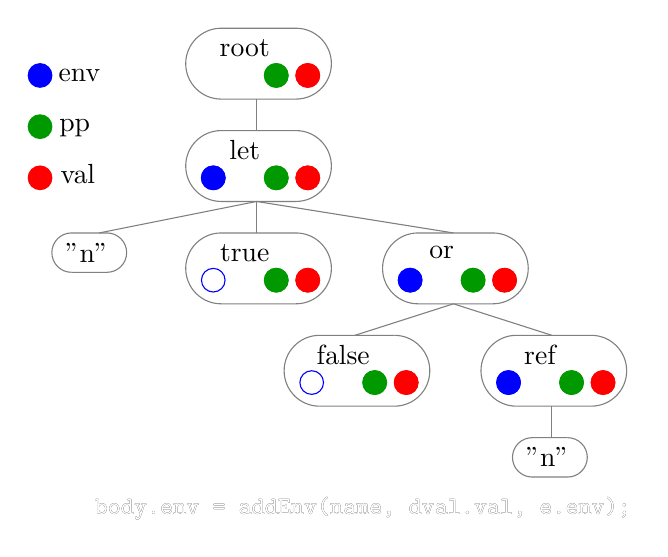
\begin{tikzpicture}

%\draw ($(5.5,\ys*-0.5)$) node {\small\texttt{body.env = addEnv(name, dval.val, e.env);}};

\envc{1.8}{4}
\draw (1.9,4.85) node{env};

\ppc{1}{3.5}
\draw (1.84,4.18) node{pp};

\valc{0.6}{3}
\draw (1.88,3.6) node{val};

\rtn{4}{4}{root}
\tedge{4}{4}{4}{3}

\tn{4}{3}{let}
\tedge{4}{3}{2.0}{2}
\tedge{4}{3}{4}{2}
\tedge{4}{3}{6.5}{2}

\tnstr{2.0}{2}{"n"}

\tn{4}{2}{true}

\tn{6.5}{2}{or}
\tedge{6.5}{2}{5.25}{1}
\tedge{6.5}{2}{7.75}{1}

\tn{5.25}{1}{false}

\tn{7.75}{1}{ref}
\tedge{7.75}{1}{7.75}{0}

\tnstr{7.85}{0}{"n"}

\ppeval

\valeval



\end{tikzpicture}
\end{frame}


\begin{frame}{Higher Order Attributes}
\biA
 \x Synthesized and inherited attributes can be \hib{syntax trees}.

 \x Such a tree can be ``rooted'' so that
  \bi
   \x by giving it inherited attributes
   \x synthesized attributes can be computed and accessed.
  \ei

 \x These were call ``nonterminal attributes'' in Vogt and Swierstra's
    original work.

   \begin{tabbing}
    \code{xx}\=\code{xx}\=\code{xx}\=\kill
    \code{production p} \\
    \code{x::X ::= y::Y z::Z  |  a::A  b::B} \\
    \code{\ttlbrace{}} \\
    \>\code{a = ... ;} \\
    \>\code{a.i = ... ;} \\
    \>\code{... = ... a.s ... ;} \\
    \code{\ttrbrace{}} 
    \end{tabbing}

\ei
\end{frame}

\begin{frame}[fragile]{Implementing \code{lookup} on \code{Env}}


Recall,
\begin{verbatim}
production ref
e::Expr := name::String
{ e.val = case lookup( name, e.env) of ...    }
\end{verbatim}

\bigskip
Here \code{lookup} is an undefined function and
%
\code{Env} is an undefined type.

\pause
\bigskip
We can instead implement this directly in the AG formalism with higher
order attributes.
\end{frame}

\begin{frame}[fragile]{Implementing \code{lookup} on \code{Env}}
\small
\begin{verbatim}
nonterminal Env;
inh attr lookup::String occurrs on Env;
syn attr result::Maybe<Boolean>
\end{verbatim}

\pause
\begin{verbatim}
production nil_Env
e::Env ::=
{ e.result = Nothing(); }

production cons_Env       {- called 'addEnv' above -}
e::Env ::= nm::String v::Boolean rest::Env
{ e.result = if nm = e.lookup then Just(v) else rest.result;
  rest.lookup = e.lookup;   }
\end{verbatim}

\pause
\begin{verbatim}
production ref
e::Expr := name::String
{ local this_env = e.env;
  this_env.lookup = name;
  e.val = case this_env.result of ...   }
\end{verbatim}

\end{frame}

\begin{frame}{Scopes}
\biA
 \x \code{Env} above was a flat list.
 \x We can build more sophisticated data structures.
 \x Binary trees for efficient lookup.
 \x Lists of lists/trees, for nested scopes.
\ei
\end{frame}



\begin{frame}{Reference attributes}
\biA
\x Can be seen as references or pointers to other decorated nodes in
the syntax tree.
\bi
 \x This make sense in an imperative setting.
\ei
\x Can also be seen as values that are decorated trees with inherited
and synthesized attributes.
 \bi
  \x This makes sense in a functional setting.
 \ei
\x See work by John Boyland and G\:orel Hedin.
\ei
\end{frame}

\begin{frame}[fragile]{Implementing \code{Env} with reference attributes}
\small
\begin{verbatim}
nonterminal Env;
inh attr lookup::String occurrs on Env;
syn attr result::Maybe<Decorated Expr>
\end{verbatim}

\pause
\begin{verbatim}
production cons_Env
e::Env ::= nm::String  b::Decorated Expr  rest::Env
{ e.result = if nm = e.lookup then Just(b) else rest.result;
  rest.lookup = e.lookup;   }
\end{verbatim}

\pause
\begin{verbatim}
production let
e::Expr ::= name::String dval::Expr body::Expr
{ body.env = addEnv(name, dval, e.env); }  {- was dval.val -}

production ref
e::Expr := name::String
{ local this_env = e.env;    this_env.lookup = name;
  e.val = case this_env.result of .
          | Just(dval) -> dval.val 
          | _ -> False    }
\end{verbatim}

\end{frame}



\begin{frame}[fragile]{New syntax = new productions}
\begin{verbatim}
grammar implication;
imports boolExprHost;
production implies
e::Expr ::=  l::Expr  r::Expr
{ e.pp = "(" ++ l.pp ++ "=>" ++ r.pp ++ ")";
  ... }
\end{verbatim}
%forwards to or( not(l), r );   }
\pause

\bigskip
Similarly, the \hib{\texttt{match}} and \texttt{datatype}
constructs add new syntax to the host language C.

\begin{tabbing}
\texttt{production \hib{match}} \\
\texttt{s::Stmt ::= scrutinee::Expr clauses::Clauses}\\
\texttt{production \hib{clause}} \\
\texttt{c::Clause ::= p::Pattern  value::Expr}
\end{tabbing}

\bigskip
This also adds new nonterminals
\texttt{\hib{Clauses}}, \texttt{\hib{Clause}}, and
\texttt{\hib{Pattern}}.

\end{frame}


\begin{frame}[fragile]{New analysis/translation = new attribute, equations}

\begin{verbatim}
grammer errors:
imports boolExprHost;

syn attr errors :: [Msg];
attr errors occurs on Root, Expr

aspect production or
e::Expr ::= l::Expr r::Expr
{ e.errors = l.errors ++ r.errors ++
    .. check that l and r are Boolean ... ;
}
\end{verbatim}

\pause
\bigskip
The Cilk extension creates an additional clone of 
\texttt{\hib{cilk}} functions.
\end{frame}


%\begin{frame}{Extensions}
%I think this goes away
%  \bi
%   \x new syntax = new productions
%   \x new semantics = new equations, in aspect productions
%  \ei
%\end{frame}


\begin{frame}[t]{Composition of AG specifications}
\begin{tabbing}
The \=``extensibility in both directions'', \\
    \>``no modification of existing code'', and \\
    \>``no linear ordering'' components.
\end{tabbing}

\bigskip
Grammar composition is simply component-wise set union.

\bigskip
Specifications are just sets of
\bi
 \x nonterminals
 \x productions
 \x equations for a production
 \x attribute declarations
 \x ...
\ei

\pause

\bigskip
But what is \code{errors} on \code{implies} ?
\end{frame}






\begin{frame}[fragile,t]{Forwarding}
The ``no glue code'' component.

{\small
\begin{verbatim}
production implies
e::Expr ::=  l::Expr  r::Expr
{ e.pp = "(" ++ l.pp ++ "=>" ++ r.pp ++ ")";
  forwards to or( not(l), r ); {- expr, not template -}  }
\end{verbatim}
}

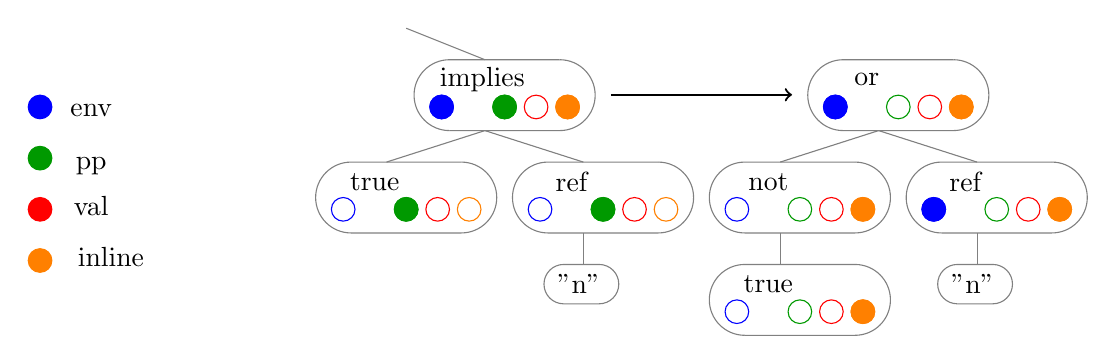
\begin{tikzpicture}
\showimplies
\end{tikzpicture}

\bigskip
Similarly for \texttt{\hib{match}} and \texttt{\hib{fastClone}}.
\end{frame}







\begin{frame}{Building language extensions in \ableC{}, an overview}

Our first foray into building language extensions will be with the
"getting-started" tutorial, found here:

\medskip
\code{ableC-bundle/ableC/tutorials/getting\_started}

\bigskip
Here we will explore the specification of
\bi
 \x concrete syntax
 \x abstract syntax
 \x translation to plain C, via forwarding
\ei

%\pause
%\bigskip
%\textbf{Exercise:}
%Extend this extension with a similar "goodbye!" construct.

%\note{Make changes inside tutorials directory for now...}
\note{\bi
\x Shows basic structure
\x Show concrete and abstract syntax
\x doesn't use silver-ableC
\ei
}
\end{frame}



\begin{frame}{Error Checking}

We next consider basic error checking in \ableC{}.  For this, we look
at an extension that adds a new operator for averaging numbers and
checks that its operands are integers.  

\bigskip
For this, look here:

\bigskip
\code{ableC/tutorials/error\_checking}

\bigskip
Here we use the use of an \code{errorExpr} production in forwarding and
some use of type representations.

%- TODO: still old-style forwarding AST specs
%  - can we use the silver-ableC version of Silver?

\note{\bi
\x Uses ``hacked'' grammar to allow new operators without
   breaking MDA.
\x (bad use of locations)
\x still no silver-ableC
\ei
}
\end{frame}


\begin{comment}
\begin{frame}{Declarations and Environments}
SKIP - nothing good to see here.

The \ableC{} environment allows extensions to add new forms of
declarations that add new name-bindings.  This is fleshed out in the
tutorial


\bigskip
\code{ableC/tutorials/declarations}

\bigskip

The \code{env} attribute is an inherited \code{autocopy} which means it is
autmatically copied down the syntax tree.

\bigskip
A \code{addEnv} production is used to add new binding into an
environment.  These are to specific namespaces:
namespaces values, tag types (structs, unions), labels, etc.


%- TODO: can we add a call to "lookup" before discussing the outputs
%  (ValueItem, etc)
  
%\bigskip
%No exercise, just take a look.
\end{frame}
\end{comment}

\begin{frame}{Embedded DSLs}
``Embedded DSLs'' are typically small domain-specific languages that
  are now part of a larger general purpose language.

\bi
 \x Consider the Halide extension
 \x Consider the tutorial \code{ableC/tutorials/embedded\_dsl}
 \bi
  \x \emph{e.g.}  \code{prefix(+ 1 - 2 * 3 / 4 5)}
 \ei
 \x Idea also seen in the SQL extension.
\ei

\bigskip
This relies on context aware scanning.
\end{frame}


\begin{frame}{Operator Overloading}
Consider the 
\code{ableC/tutorials/overloading}
examples.

\note{\bi
\x No new concrete syntax 
\x example - adds an interval type
\x concrete syntax - just stuff for the type and interval literals
\x abstract syntax - in Type.sv, we see the overloading
\x also show something in ableC?
   - abstract / overloadable / ExprBinOp.sv - line 83 - 93
\ei}
\end{frame}


%\begin{frame}{Silver - a lazy functional language}
%Consider some example of Silver, illustrating its abilities as a lazy
%functional language.
%\end{frame}


\begin{frame}{Silver-AbleC}

Writing the translations of extensions to C has been painful!
\bi
\x All those uses of abstract syntax productions...
\ei

\bigskip
A recent Silver development is a Silver extension that allows one to
write these ``forwards to'' expressions in the concrete syntax of C.

\bigskip
An exponentiation operator demonstrates this.
\end{frame}


\begin{frame}{More \ableC{} extensions}
\biA
\x Taco
\x Halide
\x Prolog
\x Limited C++ style templates
\x Go-style message passing
\x Type qualifiers, \eg{} \code{nonnull}, \code{watch}, dimension
   analysis
\ei
\note{Just show some sample bits of code from some other}
\end{frame}


\begin{frame}{Modular Analysis for Attribute Grammars}
\end{frame}


\begin{frame}[t]{Effective completeness}
\egreen{An equation exists for all attribute values that may be computed.}

\bigskip
This is the ``strong static typing'' component of the expression problem.

\bigskip
Without forwarding, completeness is easy.
 \bi
  \x Every attribute instance has a defining equation.

  \x Well-definedenss analysis adds non-circularity check.
 \ei
%      All attributes on all nodes have equations that define their
%      value.

%      May add non-circularity, but in lazy languages this is not
%      always a problem.

\bigskip
With forwarding, effective completeness
 \bi
  \x Every attribute instance that is used has a defining equation.

  \x Some inherited attribute equations are not needed.

  \x \eg\ \code{env} on children of \code{implies} on previous slides.
 \ei
\end{frame}



\begin{frame}[t]{Modular effective completeness}
The ``separate type checking'' component.

\bigskip

$\mathit{complete} ( H \cup \{ E_1, ... , E_n \} ) $ \ \ ?

%\pause
\bigskip

$\forall i \in [1,n] . \mathit{modComplete}(H, E_i) 
 \Rightarrow \mathit{complete}( H \cup \{ E_1, ..., E_n \} )$

\bigskip
In three parts:
\be
 \x well-formedness
 \x synthesized completeness
 \x effective inherited completeness
\ee
\end{frame}

\note{Can be extended to modular circularity, but Silver is lazy and
  thus cycles are not always bad and are sometime used.}


\begin{frame}[t]{Well-formedness (1/2): orphaned occurs}

\begin{tabular}{rcl}
$G_{nt}$   & : & \texttt{nonterminal Expr;} \\
$G_{attr}$ & : & \texttt{syn attr errors ::\ [Msg];}\\
$G_{occ}$  & : & \texttt{attr errors occurs on Expr;}
\end{tabular}

\bigskip
Require occurs-on declaration is in $G_{nt}$ or $G_{attr}$.

\bigskip
Ensure at most one such declaration.
\be
 \x $G_{nt} = G_{attr} = G_{occ}$ - \eg\ \texttt{val}
 \x $G_{nt} = G_{occ}$ and imports $G_{attr}$ 
 \x $G_{attr} = G_{occ}$ and imports $G_{nt}$ - \eg\ \texttt{errors}
\ee
\end{frame}


\begin{frame}[t]{Well-formedness (2/2): orphaned equations}

\begin{tabular}{rcl}
$G_{p}$   & : & \texttt{production and} \\
          &   & \texttt{e::Expr ::= l::Expr r::Expr \ttlbrace ...\ttrbrace} \\
$G_{occ}$ & : & \texttt{attr errors occurs on Expr;}\\
$G_{eq}$  & : & \texttt{aspect production and } \\
         &   & \texttt{e::Expr ::= l::Expr r::Expr } \\
         &   & \texttt{\ttlbrace e.errors = ...; \ttrbrace} 
\end{tabular}

\bigskip
Require equation is in $G_p$ or $G_{occ}$.

\bigskip
Ensure at most one equation.
\be
 \x $G_{p} = G_{occ} = G_{eq}$ - \eg\ \texttt{val} in host
 \x $G_{p} = G_{eq}$ and imports $G_{occ}$ - \eg\ \texttt{implies}
 and \texttt{pp}
 \x $G_{occ} = G_{eq}$ and imports $G_{p}$ - \eg\ \texttt{errors} 
\ee
\end{frame}


\begin{frame}{Syn completeness (1/2): orphaned productions}

Requires a production with host language nonterminal is 
\bi
 \x in host language grammar
 \x or it forwards
\ei

\begin{alltt}
\begin{tabbing}
aaaaaaaaaaaaaaaaaaaaaaaaaa\=aa\=\kill
grammar boolExprHost;
\>grammar implication; \\

\\

nonterminal Expr;
\>production implies \\

\>e::Expr ::= ... \\

production and  
\>\ttlbrace\>... \\

e::Expr ::= ... 
\>\>forwards to ... \ttrbrace \\

\ttlbrace\ \ ... \ttrbrace \\


\>\hir{production xor} \\
\>\hir{e::Expr ::= ...} \\
\>\hir{\ttlbrace\ ... no forwarding ... \ttrbrace}
\end{tabbing}
\end{alltt}


\bigskip
Note the \texttt{Pattern} nonterminal in inductive types extension need
not forward.
\end{frame}


\begin{frame}[t]{Syn completeness (2/2): occurs check}
\begin{tabbing}
$G_{occ}$\ :\  \texttt{attr errors occurs on Expr;}
\end{tabbing}

\bigskip
Require the \emph{occurs-on} declaration can check that all non-forwarding
productions with lhs of \texttt{Expr} have equation for
\texttt{errors}. 

\bigskip
This relies on no orphaned productions condition.

\bigskip
Both ensure that forwarding is used properly and that only ``local''
checks needed for synthesized completeness.
\end{frame}


\newcommand{\errorevalnoanim}{
\ppc{6.5}{2} %implies

\ppc{5.25}{1} % imp-true
\ppc{7.75}{1}% imp-ref

\errd{6.5}{2} %implies

%\errd{5.25}{1} % imp-true
%\errd{7.75}{1}% imp-ref

\errd{11.5}{2} % or
\errd{10.25}{1} % not
\errd{10.25}{0} % or-true

\errc{10.25}{0} % or-true
\errc{10.25}{1} % not

\errd{12.75}{1} % or-ref
\envd{12.75}{1} % or-ref
\envd{11.5}{2} % or

\envd{6.5}{2} %implies
\envc{6.5}{2} %implies

\envc{11.5}{2} % or

\envc{12.75}{1} % or-ref
\errc{12.75}{1} % or-ref

\errc{11.5}{2} % or

\errc{6.5}{2} %implies
}

\newcommand{\showimpliesnoanim}{
\ifthenelse{\boolean{showanim}}{\errc{3.5}{0}\draw (5.5,-0.35) node{errors};}{}

\tedge{5.5}{3}{6.5}{2}
\tne{6.5}{2}{\ \ implies}
\tedge{6.5}{2}{5.25}{1}
\tedge{6.5}{2}{7.75}{1}

\draw[thick,->] ($(8.25,\ys*1.85)$) -- ($(10.55,\ys*1.85)$);

\tne{5.25}{1}{true}

\tne{7.75}{1}{ref}
\tedge{7.75}{1}{7.75}{0}

\tnstr{7.85}{0}{"n"}


\tne{11.5}{2}{or}
\tedge{11.5}{2}{10.25}{1}
\tedge{11.5}{2}{12.75}{1}

\tne{10.25}{1}{not}
\tedge{10.25}{1}{10.25}{0}

\tne{10.25}{0}{true}

\tne{12.75}{1}{ref}
\tedge{12.75}{1}{12.75}{0}

\tnstr{12.85}{0}{"n"}

\errorevalnoanim
}

\begin{frame}{Effective inherited completeness}

\setboolean{showanim}{false}
\begin{tikzpicture}[scale=0.7, every node/.style={scale=0.7}]
\showimpliesnoanim
\end{tikzpicture}


\begin{alltt}
\begin{tabbing}
aa\=\kill
production implies  e::Expr ::=  l::Expr  r::Expr \\
\ttlbrace e.pp = ... ; \\
\>forwards to or( not(l), r ); \\
\ttrbrace
\end{tabbing}
\end{alltt}

No need to define \texttt{env} on \texttt{l} or \texttt{r}
since \texttt{val} computed on forwards to tree.
\end{frame}

\newcommand{\tname}[3]{
\draw[gray] ($(#1,#2*\ys)$) node{#3};
\draw[gray] ($(#1+0.4,\ys*#2+0.25)$) --
            ($(#1-0.4,\ys*#2+0.25)$) arc (90:270:2.5mm);

\draw[gray] ($(#1+0.4,\ys*#2+0.25)$) arc (90:-90:2.5mm) -- 
            ($(#1-0.4,\ys*#2-0.25)$) ;

}

\begin{frame}[t]{Flow types}
Record attribute dependencies. \ \ \hib{They are inferred.}

\bigskip
$ft_{Expr}(pp) = \{ \}$  \ \ \ 
%
$ft_{Expr}(val) = \{ env \}$ \ \ \ 
%
$ft_{Expr}(fwd) = \{ \}$ \\
\ \ \  {\small (but in richer languages $ft_{Expr}(fwd)$ often includes \texttt{env})}

\bigskip
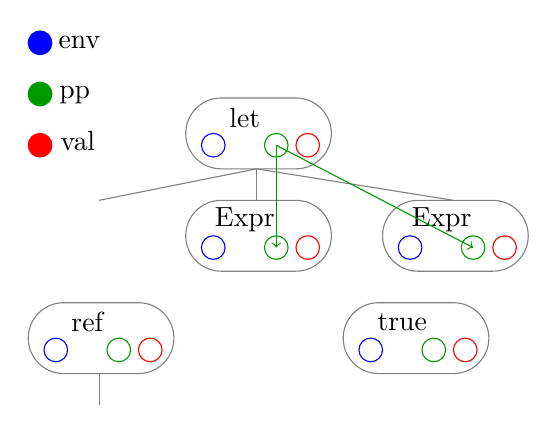
\begin{tikzpicture}
\envc{1.8}{4}
\draw (1.9,4.85) node{env};

\ppc{1}{3.5}
\draw (1.84,4.18) node{pp};

\valc{0.6}{3}
\draw (1.88,3.6) node{val};


\tn{4}{3}{let}
\tedge{4}{3}{2.0}{2}
\tedge{4}{3}{4}{2}
\tedge{4}{3}{6.5}{2}

\tname{2.0}{2}{String}
\tn{4}{2}{Expr} %dval
\tn{6.5}{2}{Expr} %body

\tn{2}{1}{ref}
\tedge{2}{1}{2}{0}
\tname{2}{0}{String}

\tn{6}{1}{true}


\pause
\pptopp{4}{3}{4}{2}
\pptopp{4}{3}{6.5}{2}

\end{tikzpicture}

\end{frame}

\begin{frame}[t]{Flow types}
Record attribute dependencies. \ \ \hib{They are inferred.}

\bigskip
$ft_{Expr}(pp) = \{ \}$  \ \ \ 
%
$ft_{Expr}(val) = \{ env \}$ \ \ \ 
%
$ft_{Expr}(fwd) = \{ \}$ \\
\ \ \  {\small (but in richer languages $ft_{Expr}(fwd)$ often includes \texttt{env})}

\bigskip
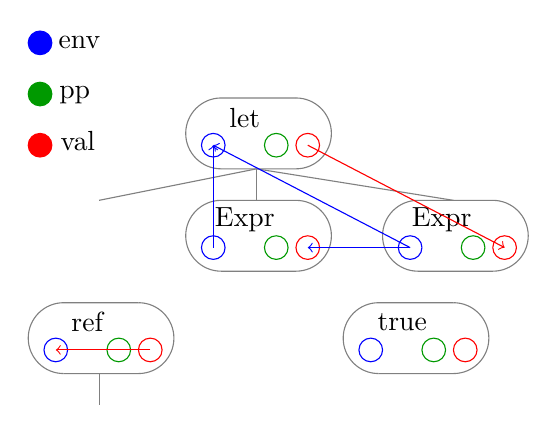
\begin{tikzpicture}
\envc{1.8}{4}
\draw (1.9,4.85) node{env};

\ppc{1}{3.5}
\draw (1.84,4.18) node{pp};

\valc{0.6}{3}
\draw (1.88,3.6) node{val};


\tn{4}{3}{let}
\tedge{4}{3}{2.0}{2}
\tedge{4}{3}{4}{2}
\tedge{4}{3}{6.5}{2}

\tname{2.0}{2}{String}
\tn{4}{2}{Expr} %dval
\tn{6.5}{2}{Expr} %body

\tn{2}{1}{ref}
\tedge{2}{1}{2}{0}
\tname{2}{0}{String}

\tn{6}{1}{true}

\pause
\valtoenv{2}{1}{2}{1} % body -> body

\pause

% let.val -> body.val
\valtoval{4}{3}{6.5}{2}


%\pause
% body.val -> body.env
% \valtoenv{6.5}{2}{6.5}{2} % body -> body


\pause
\envtoenv{6.5}{2}{4}{3} % body -> let
\pause
\envtoval{6.5}{2}{4}{2} % body -> dval


% \valtoenv{4}{2}{4}{2} % dval -> dval
\pause
\envtoenv{4}{2}{4}{3} % dval -> let


%\valtoval{4}{3}{4}{2}


\end{tikzpicture}

\end{frame}


\begin{frame}[t]{Effective inh. completeness (1/2): modularity}
\bis{0.8cm}
\x Compute flow types for host $H$: $ft^H$ 

   and then again for extension $H \triangleleft E$: $ft^E$.

\x For each synthesized attribute occurrence in $H$

   ~~~~~~~~~~~~$ft^H_{nt}(s) = ft^E_{nt}(s)$.

 \bi
  \x Extensions can't add more dependencies.
  \x Also, $ft^H_{nt}(fwd) = ft^E_{nt}(fwd)$.
 \ei

\x For each synthesized attribute occurrence in $E$,\\

   ~~~~~~~~~~~~$ft^H_{nt}(fwd) \subseteq ft^E_{nt}(s)$.

 \bi
  \x May need to evaluate forward equations.
 \ei
\ei
\end{frame}


\begin{frame}[fragile,t]{Effective inh. completeness (2/2): checks}
For each synthesized attribute access, \\
check that the necessary inherited equations are supplied.

\begin{verbatim}
production implies
e::Expr ::=  l::Expr  r::Expr
{ e.pp = "(" ++ l.pp ++ "=>" ++ r.pp ++ ")";
  forwards to or( not(l), r );   }
\end{verbatim}

\pause
Erroneously, define without defining \texttt{env}

\begin{verbatim}
production implies
e::Expr ::=  l::Expr  r::Expr
{ e.pp = "(" ++ l.pp ++ "=>" ++ r.pp ++ ")";
  e.val = if l.val then r.val else false ; }
\end{verbatim}

\end{frame}


\begin{frame}[t]{Summarize}

$\forall i \in [1,n] . \mathit{modComplete}(H, E_i) 
 \Rightarrow \mathit{complete}( H \cup \{ E_1, ..., E_n \} )$

   \bi
    \x every grammar agrees on $ft_{nt}(s)$ when it knows about $nt$
    and $s$.

    \x inherited equations supplied when needed

    \x check is local to the grammar
   \ei

There is a faster algorithm that doesn't generate flow types for both
$H$ and $H \triangleleft E_i$.
\end{frame}


\begin{frame}[t]{Ramifications of modular composable language design}
\biA
 \x There is a difference between composable extensions and language
    modifications.

\pause
 \bis{0.3cm}
 \x Need a rich host language to ensure extensions can be specified in
    it.

 \x Modular analysis is not reasonable in early stages of development.
 
 \x These points hold for both concrete syntax and static analysis.
 \ei

\pause
 \x Our experience shows (and our biases claim) that we can answer
 ``yes'' 

  to our 4 questions.

\be
\x Can programming languages be constructed from composable modules, \\
   each defining an extension to a host language?

\x Can extensions add new syntax and new static semantics?

\x Can extension be developed independently?

\x Can programmers compose the extensions of their choosing \\
   \underline{without} needing to understand the underlying
   implementations?
\ee
\ei
\end{frame}


\begin{comment}
\begin{frame}[fragile]{Extending a map/fold example}

For the remainder of our time we have prepared a simple map/fold
extension that you may extend to learn more about \ableC{} and
\silver{}.

\bigskip
\begin{lstlisting}
\% cd PPoPP/ableC-bundle/extensions

\% git clone https://github.com/melt-umn/ableC-mapFold-exercise

\% cd ableC-mapFold-exercise/examples

\% more map\_fold.xc
\end{lstlisting}
\end{frame}
\end{comment}

%\begin{frame}{Other uses}
%\bi \x End-user developed DSLs \ei
%\end{frame}
%\note{This is the place for the meme.}


\begin{frame}{Future Work}
\biA
 \x Continued work on ableC, Copper, Silver

 \x Parallel evaluation of AGs

 \x Modular verification of meta-theoretic properties
  \bi
   \x nicer looking specifications, easier to reason about

   \x using a notion of implicit monads to mimic SOS style rules in
      AGs ... tomorrow.
  \ei
\ei
\end{frame}


\begin{frame}
\begin{center}
Thanks for your attention.

\vskip 1cm
Questions?

\vskip 1cm

\code{http://melt.cs.umn.edu} \ \ \ \ 
\code{evw@umn.edu}
\end{center}
\end{frame}


\begin{frame}{Additional Slides}

\vskip 0.6cm
The details of modular determinism analysis.

\vskip 1cm
Determinism
\bi
\x in the parser: no conflicts
\x in the scanner: no overlapping regexs
\ei
\end{frame}


\begin{frame}{LR parsing tables and conflicts}
\biA
 \x Parser actions are typically organized into a table:
   \bi
    \x states on one axis, terminals one another
    \x the action is the table cell entry
  \ei
\x During table construction, some grammars will result in more than
one action in an entry.

\x This is called a \ered{conflict}.  The grammar is not LALR(1).
 \bi \x It  cannot be parsed by a LALR(1) parser.
 \ei

\x Grammars whose tables have no conflicts are \eblue{deterministic}.

\x We want deterministic grammars.

\x The check for no conflicts is, in effect, a \eorange{determinism analysis}.
\ei
\end{frame}


\begin{frame}{Syntactic determinism and context aware scanning}
\biA
 \x Context-aware scanning uses the same determinism analysis.

 \x Note: the parser only sees terminal names, not their regexs.

    \bigskip
    Thus, the two ``table'' terminals are different, from the
    perspective of the parser.

 \x Without context-aware scanning they would need to be the same
 terminal.

 \x This may introduce conflicts that do not arise in context-aware scanning.
\ei
\end{frame}

\begin{frame}{Lexical determinism and context aware scanning}
\bi
 \x Ensure that the scanner will never return more than one terminal
 symbol on the same input.

 \x An analysis for lexical determinism:

   % \x no conflicts in parse table   syntactic determinism
    \begin{tabbing}
       for \=each parse state $p$,  \\
	   \>for each pair of distinct terminals $t_1$, $t_2$,\\
           \>\ \  both in valid-lookahead(p), \\
           \> $t_1$ and $t_2$ regexs must be disjoint languages 
              \eorange{(no overlap)}\\
	   \>or\\
           \>( $t_1 > t_2$   or   $t_2 > t_1$ )
             \eorange{(disambiguation by lexical precedence)}
       \end{tabbing}
     This implies lexical determinism.
 \ei
\end{frame}

\begin{frame}{Monolithic analyses}
\biA
 \x This syntactic determinism analysis and
    lexical determinism analysis
  \bi
   \x \eblue{examine the entire composed grammar}
   \x and ensure that a correct parser and scanner can be generated.
  \ei

 \x These are important.

 \x But, they must be done on the composed grammar.

 \x Recall our goal of programmer-directed language composition.
\ei
\end{frame}







\begin{frame}{Composition of Deterministic Grammars}
Solution uses standard LALR(1) parsing
with some modifications:
\bis{0.3cm}
\x naming techniques
 \bi \x so that the parser sees terminals and non-terminals defined in
     different extensions as being different.  
 \ei
\x context-aware scanning 
 \bi \x  makes it practical
 \ei
\x restrictions on grammars
\x limited but natural lexical disambiguation by programmer
  \bi \x similar to using fully qualified names in Java to
  disambiguate class names
  \ei
\ei
\end{frame}


\begin{frame}{Specifications}
\bi
\x host language specification - defines a complete language
\bi
 \x terminals (with regexs), non-terminals, productions ...
% \x terminals associated with regexs
% \x lexical and operator precedence are also supported
\ei
\pause
\x language extension specification
\bi
 \x defines new terminals, non-terminals, productions
 \x but may reference those defined in the host language
 \x $\nt{expr}\ ::=\  \term{DNF\_table} \ '('\ \nt{tableRows}\ ')'$ \\
    $\nt{tableRow}\ ::=\ \nt{expr}\ ':'\ \nt{tfstarList}$
\ei
\pause
\x full names based on grammar name and construct name
\bi
 \x \texttt{edu:umn:cs:melt:ableJ:Expr}
 \x \texttt{edu:umn:cs:melt:ableJ:exts:tables:table}
 \x \texttt{org:someone:extensions:sql:table}
\ei
\x composition is just component-wise union of grammars 
\ei
\end{frame}


\begin{frame}{Modular determinism analysis}

\bis{0.3cm}
 \x {\large $CFG_C = CFG^H \cup^* \{ CFG^{E_1}, ... , CFG^{E_n} \}$}
 \x 
{\large
\begin{tabbing}
  \only<1->{$\forall i \in [1,n]\ .$}\ \= 
     \only<1->{$\mathit{isComposable}(CFG^H, CFG^{E_i})\ \ \ \land$} \\
 \>  \only<1->{$\mathit{conflictFree}(CFG^H \cup CFG^{E_i})$}  \\

 \only<1->{$\Rightarrow \mathit{conflictFree}(CFG^H \cup \{ CFG^{E_1},
   ... , CFG^{E_n} \})$} 
\end{tabbing}
}

 \x \eblue{isComposable} is an analysis that the language extension designer can run.
 \x It certifies individual extensions with the host language.
 \x All certified extension grammars can be be composed - to form a
 deterministic grammar.
\ei
\end{frame}

\begin{frame}{Partitioning of Host-and-2-exts LR-DFA}
  \epsfysize=0.5\linewidth
  \epsffile{images/Host_and_two.pdf}   
\end{frame}


\begin{frame}{What is and is not allowed}
\bis{0.3cm}
\x Extension constructs can contain host language constructs.
\bi
 \x ext. productions have host NTs on right hand side
 \x the tables construct contains host language expressions
\ei
\x Few restrictions (beyond LALR(1) restrictions) on embedded languages
 \bi \x e.g. SQL \ei
\x Restriction types:
 \bi \x on grammar structure, 
     \x on grammar properties (follow sets), and
     \x on the LR DFA
 \ei
\ei
\end{frame}


\begin{frame}[fragile]{Restriction 1: grammar structure}
\bis{0.3cm}
\x \eorange{``marking terminal''}
 \bi 
  \x an extension production with a host language nonterminal on
     the l.h.s. must have a right hand side that begins with a
     ``marking  terminal'' 
  \x these are called \eorange{``bridge productions''}
 \ei

\x \eblue{$\nt{expr}\ ::=\ \term{DNF\_table} \ '('\ \nt{tableRows}\ ')'$}

   \eblue{$\nt{tableRow}\ ::=\ \nt{expr}\ ':'\ \nt{tfstarList}$}

\x 
\begin{verbatim}
b = table ( age > 40      : T * ,
            gender == "M" : T F ) ;
\end{verbatim}

\x Transition from host state to extension state only by shifting a
marking token.
\ei
\end{frame}


\begin{frame}{Restriction 2: follow sets}
\bis{0.3cm}
\x In the combined host language and single extension grammar 
   $(\Gamma^H \cup_G \Gamma^{E_i})$,

   no new terminals added to the follow sets of host language
   non-terminals, except for marking terminals.

\x \eblue{$\nt{expr}\ ::=\ \term{DNF\_table} \ '('\ \nt{tableRows}\ ')'$}

   \eblue{$\nt{tableRow}\ ::=\ \nt{expr}\ ':'\ \nt{tfstarList}$}

\x follow set of \eblue{$Expr$} already contained ‘:’
\x Extensions are more easily added to languages with larger follow sets.
\ei
\end{frame}


\begin{frame}{Restriction 3: LR DFA}
\bis{0.2cm}
\x partition the LR DFA of $(\Gamma^H \cup_G \Gamma^{E_i})$ to
   maintain determinism
\x host language states are those with items that only use host
   language terminals or nonterminals
 
   \eg\  $\nt{stmt}\ ::=\ '\texttt{while}' \ '('\ \bullet\ \nt{expr}\ ')'\ \nt{stmt}$

\x except that they can be extended in the LR DFA of 
   $(\Gamma^H \cup_G \Gamma^{E_i})$ in limited ways 
 \bi
   \x only marking terminals can be added to their item’s lookahead 
   \x new items must be bridge productions;

      these have the form $\nt{H} ::= \bullet\ \mu\ ...$ where $\mu$ is a marking terminal
  \ei

\x host language states $s$ in LR-DFA $(\Gamma^H \cup_G \Gamma^{E_i})$ 
   and not in LR-DFA $(\Gamma^H)$ are 

   such that their items and lookahead are the subsets of those of a
   state in 

   LR-DFA $(\Gamma^H)$ (called ``new host'' states).

\ei
\end{frame}


\begin{comment}
\begin{frame}{Partitioning of Host-and-1-ext LR-DFA}
%c\\begin{center}
  \epsfysize=0.65\linewidth
  \epsffile{images/Host_and_one.pdf}   
%\end{center}
\end{frame}
\end{comment}



\begin{frame}{Modular Lexical Determinism Analysis}

Partition of parser DFA ensures that lexical ambiguities are
\eblue{only} between 

\bi
 \x terminals in host and a single extension,
   \bi \x these are resolved by extension writer \ei
\pause
 \x or between marking terminals on two different extensions
 \bi
  \x cannot be resolved by extension writer
  \x only programmer who composed the language can resolve them.
  \x accomplished by \eorange{transparent prefixes}

     \texttt{b = :edu:umn:cs:melt:ableJ:exts:table ( ... }
 \ei
\ei
\end{frame}

\begin{frame}{Experience with restrictions}
\bis{0.3cm}
 \x SQL, tables, various others all pass easily.
 \x Most were developed before this analysis.

 \x Recall:

   \eblue{$\nt{expr}\ ::=\ \term{DNF\_table} \ '('\ \nt{tableRows}\ ')'$}

   \eblue{$\nt{tableRow}\ ::=\ \nt{expr}\ ':'\ \nt{tfstarList}$}

\x follow set of \eblue{$\nt{expr}$} already contained ‘:’
\x Extensions are more easily added to syntactically rich languages.

   This is because they have larger follow sets.

   Not so easy on small ``toy'' language
\ei
\end{frame}


\begin{frame}{Restrictions and new infix operators}
Grammars that add new infix operators for host language expressions
do not pass the modular analysis. 
\bis{0.3cm}
 \x Embedded language can define new infix operators.
 \x The SQL extension does this – this is allowed.
 \x ableC has an $\nt{additiveOperator}$ nonterminal that can be
    extended. 
\ei
\end{frame}


\begin{frame}{Restrictions and AspectJ}
Java 1.4 +  abc grammar for AspectJ
\bi
 \x declarative specification for a deterministic scanner and parser
\ei
This fails the modular analysis
\bi
 \x it adds to follow sets of Java 1.4
 \x marking terminals in the wrong place
  \bi
   \x Java:    \eblue{$\nt{dcl}\ ::= \ \nt{modifiers}\ \nt{type}\ \term{Id}$}
   \x AspectJ: \eblue{$\nt{dcl}\ ::= \ \nt{modifiers}\ \nt{aspect}$}
   \x AspectJ: \eblue{$\nt{aspect}\ ::=\  'before'\ ...$}
  \ei
 \x Can refactor the host grammar to fix this problem.
\ei
\end{frame}


\end{document}

\begin{frame}{Expressiveness versus safe composition}
Compare to
\bi \x other parser generators
    \x libraries
\ei
The modular compositionality analysis does not require context aware
scanning.

But, context aware scanning makes it practical.
\end{frame}

\begin{frame}{Tool Support}
Copper – context-aware parser and scanner generator
\bi
 \x implements context-aware scanning for a LR parser
 \x lexical precedence 
 \x parser attributes
 \x disambiguation functions – when disambiguation by context and lexical precedence is not enough
 \x currently integrated into Silver
 \x also a stand alone version
 \x generated parser and scanner in Java
\ei
\end{frame}




\begin{frame}{Halide, with more cores}
\begin{alltt}
\begin{tabbing}
\hib{cs-coldpress:}\hig{examples evw}\$ ./matmul.out  \\
Building input matrices... \\
Performing matrix multiplication... 2.847800 seconds \\
Performing reference matrix multiplication... 13.592258 seconds \\
Checking results are equal... pass \\
\hib{cs-coldpress:}\hig{examples evw}\$ 
\end{tabbing}
\end{alltt}
\end{frame}





\end{document}





\documentclass[12pt]{beamer}
%\documentclass[12pt,notes=only,handout]{beamer}
%\documentclass[12pt,handout]{beamer}

\usepackage{verbatim,amssymb,ifthen,alltt,xcolor,graphicx}
\usepackage{tikz}
\usetikzlibrary{calc}
%\usetikzlibrary{calc}
%\usepackage{qtree}
\usepackage{bcprules}

\usepackage{listings}
\usepackage{multicol}

\usepackage{epsfig}
\usetikzlibrary{calc}

\usepackage{fancyvrb}
\usepackage{color}



%%-----------------------------------------
%% Shortcuts ...
%%-----------------------------------------
\newcommand{\bi}{\begin{itemize}}
\newcommand{\ei}{\end{itemize}}

\newcommand{\be}{\begin{enumerate}}
\newcommand{\ee}{\end{enumerate}}

\newcommand{\x}{\item}
%%-----------------------------------------
\newcommand{\eedd}{\end{document}}

\newcommand{\isize}[1]{\setlength{\itemsep}{#1}}

\newcommand{\bis}[1]{\begin{itemize}\setlength{\itemsep}{#1}}
\newcommand{\bes}[1]{\begin{enumerate}\setlength{\itemsep}{#1}}


\newcommand{\biA}{\bis{0.5cm}}
\newcommand{\biB}{\bis{0.65cm}}
\newcommand{\biC}{\bis{0.8cm}}
\newcommand{\biZ}{\bis{0cm}}
\newcommand{\beA}{\bes{0.5cm}}
\newcommand{\beB}{\bes{0.65cm}}
\newcommand{\beC}{\bes{0.8cm}}

\newcommand{\myitem}[2]{\item{#1}\note[item]{#2}}


\setbeamerfont{itemize/enumerate body}{}
\setbeamerfont{itemize/enumerate subbody}{size=\normalsize}
\setbeamerfont{itemize/enumerate subsubbody}{size=\normalsize}


\newcommand{\eg}{\emph{e.g.}}

\newcommand\vskipA{\vskip 0.5cm}
\newcommand\vskipB{\vskip 0.75cm}


%\newcommand{\alert}[1]{\textbf{#1}}
\newcommand{\triple}[3]{\ensuremath{\{#1\}}\ \code{#2}\ \ensuremath{\{#3\}}}

%% Symbols
\newcommand{\ttlbrace}{\mbox{\tt\symbol{123}}}
\newcommand{\ttrbrace}{\mbox{\tt\symbol{125}}}
\newcommand{\ttlbracket}{\mbox{\tt\symbol{133}}}
\newcommand{\ttrbracket}{\mbox{\tt\symbol{135}}}
\newcommand{\ttbackslash}{\mbox{\tt\symbol{92}}}
\newcommand{\tthat}{\mbox{\tt\symbol{94}}}
\newcommand{\ttat}{\mbox{\tt\symbol{64}}}
\newcommand{\tttilde}{\mbox{\tt\symbol{126}}}
\newcommand{\kwd}[1]{\textbf{#1}}

\newcommand{\back}{\ensuremath{\backslash}}
\newcommand{\defas}{\triangleq}


%% Counters
\newcounter{backupcounter}
\newcounter{exercounter}
\setcounter{exercounter}{0}



%% Colors
\setbeamercolor{redcolor}{fg=red}
\newcommand{\hir}[1]{{\usebeamercolor[fg]{redcolor}#1}}


\setbeamercolor{bluecolor}{fg=blue}

\definecolor{dgreen}{rgb}{0.0,0.6,0.0}
\definecolor{dblue}{rgb}{0.0,0.0,1.0}
\definecolor{whilte}{rgb}{0.0,0.0,0.0}

%\newcommand{\hib}[1]{{\usebeamercolor[fg]{bluecolor}#1}}

\newcommand{\hib}[1]{{\textcolor{dblue}{#1}}}
\newcommand{\hig}[1]{{\textcolor{dgreen}{#1}}}
\newcommand{\hiw}[1]{{\textcolor{white}{#1}}}

%\newcommand{\code}[1]{\texttt{\usebeamercolor[fg]{bluecolor}#1}}
%\newcommand{\code}[1]{\texttt{\hig{#1}}}
\newcommand{\code}[1]{\texttt{\hib{#1}}}
\newcommand{\nt}[1]{\ensuremath{\langle\mathit{#1}\rangle}}
\newcommand{\term}[1]{\ensuremath{\mathit{#1}_t}}
\newcommand{\termlit}[1]{``\ensuremath{\mathit{#1}}''}

%\newcommand{\frametitle}[1]{}

%\newcommand{\ftitle}[1]{\renewcommand{\frametitle}{#1}}

%% Environments - default setting, modified in
%% task_(screen|guide|notes).tex



\newcommand{\pnum}{Slide \#\arabic{framenumber}}
\newcommand{\nonotes}{\note{\pnum{} No notes for this slide}}
\newcommand{\guideonly}[1]{\mode<handout>{#1}}

%\newcommand{\

\newenvironment{exercise}[1]{\stepcounter{exercounter}%
    \begin{frame}[containsverbatim,t]{Exercise \#\arabic{exercounter}: #1}}{\end{frame}}

%\newenvironment{exercise}[1]{\stepcounter{exercounter}%
%    \begin{frame}<beamer|notes>[t]{Exercise \#\arabic{exercounter}:#1}}{\end{frame}}


% set up footer with frame number
\setbeamertemplate{footline}[text line]{%
 \parbox{\linewidth}{\vspace*{-8pt}\hfill\insertframenumber}}

% hide those navigation symbols
\setbeamertemplate{navigation symbols}{} 


%
% Note page template
% ---- ---- --------
%
\setbeamertemplate{note page}{%
%\begin{minipage}[c]{0.6\textwidth}

\textbf{Note.} \hib{\insertframetitle{}}
\insertframenumber{} / \inserttotalframenumber 

%\end{minipage}
%\begin{minipage}[c]{0.39\textwidth}
%\insertslideintonotes{0.5}
%\end{minipage}

%\begin{figure}
%\insertslideintonotes{0.25}
%\end{figure}

% 720p in 3-111
% 12x8 in Tate

%{\footnotesiz

\insertnote

}

\newcommand{\nonote}{\note{No Note. \\ \insertslideintonotes{0.85}}}
\newcommand{\stopcounting}{\setcounter{backupcounter}{\value{framenumber}}}
\newcommand{\startcounting}{\setcounter{framenumber}{\value{backupcounter}}}


\setbeamertemplate{footline}
{
  \leavevmode%
  \hbox{%
  \begin{beamercolorbox}[wd=.25\paperwidth,ht=2.25ex,dp=1ex,center]{author in head/foot}%
    \usebeamerfont{author in head/foot}%\copyright\ Eric Van Wyk
  \end{beamercolorbox}%
  \begin{beamercolorbox}[wd=.5\paperwidth,ht=2.25ex,dp=1ex,center]{title in head/foot}%
    \usebeamerfont{title in head/foot}%December 13, 2010, Braga
  \end{beamercolorbox}%
  \begin{beamercolorbox}[wd=.25\paperwidth,ht=2.25ex,dp=1ex,right]{date in head/foot}%
    % \usebeamerfont{date in head/foot}\insertshortdate{}\hspace*{2em}
%     \insertframenumber{} / \inserttotalframenumber 
     \hspace*{2ex}
  \end{beamercolorbox}}%
  \vskip0pt%
}






-- Slides --

Slides 1 or so - image of the Knuth paper
